In order to have a robust background prediction over all analysis bins, it is 
necessary to individually estimate the various background components since 
the composition is expected to vary dramatically in various bins (Figure \ref{fig:supp_Sim_Pie_lowMET}).
Low \ptmiss regions have more \gjets background, high \ptmiss regions with low \nj or \nb
is dominated by processes involving Z or W, and the high \ptmiss, high \nj, high \nb region is
mainly \ttjets or \ttg dominated.
\begin{figure}[h!]
\centering
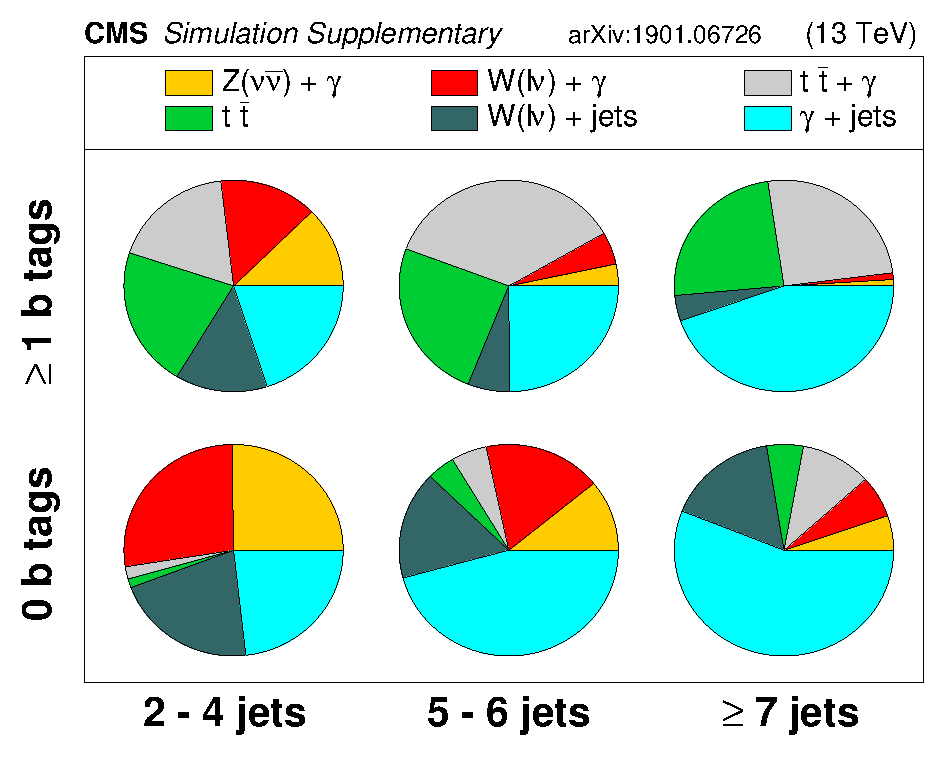
\includegraphics[width=0.48\linewidth]{../Figures/Chap3/anaPublic/supp_Sim_Pie_lowMET}
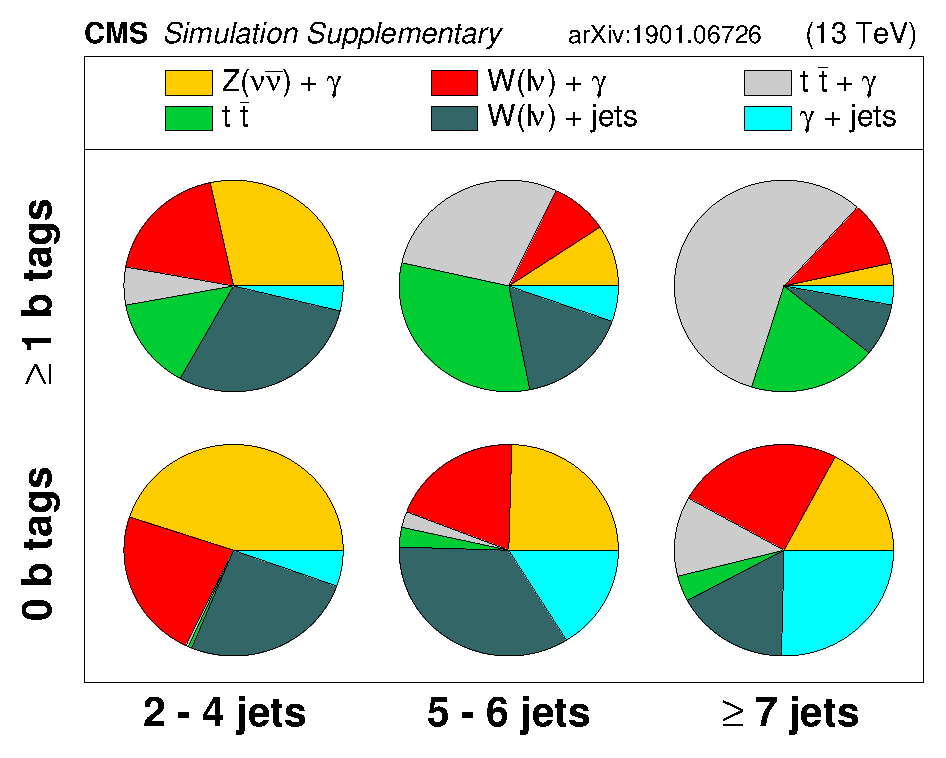
\includegraphics[width=0.48\linewidth]{../Figures/Chap3/anaPublic/supp_Sim_Pie}
\captionsetup{width=.9\linewidth}
\caption[Pie charts showing BG in low \ptmiss]{Pie charts showing relative background composition in various \nj and \nb regions for \ptmiss of 200 - 350 \gev on left and $\ptmiss\geq 350$ \gev on right.}
\label{fig:supp_Sim_Pie_lowMET}
\end{figure}

There are four main sources of background events:  events with a lost lepton (lost e/$\mu$) or a hadronically 
decaying tau leptons, events in which an electron from a $W\rightarrow e \nu$ decay fakes a photon,
$Z\rightarrow \nu \bar{\nu}$ events produced in association with a $\gamma$, and fake \ptmiss events. 

The lost lepton background arises from events in which the charged lepton
from a leptonically decaying W, produced directly or from the decay of 
a top quark, fails to be identified by being out of acceptance, 
or failing the identification or isolation requirements.  For example, in events
with high \pt top quarks, the top quark decay products will be collimated, forcing the b-jet
to be closer to the charged lepton.  In these cases, events are more likely to 
fail the isolation requirements.  These events are estimated by studying events
with both a  well-identified photon and lepton ($e/\mu$) in both data and simulation.  

The hadronic-$\tau$ background arises from events in which $\tau$ leptons from 
W decays decay to mesons and neutrinos, which occurs $\sim 65\%$ of the time.  
Due to lepton universality, the fraction of hadronically decaying $\tau$ events 
can be estimated from single muon after correcting for reconstruction differences
and for the hadronic-$\tau$ branching fraction.  

Fake photon events primarily arise from electrons from W decays faking 
photons.  This can happen when a pixel seed fails to be associated with
the photon candidate.  Given a fake rate, which relates events with well-identified
electrons with events with well-identified photons, the fake photon background
can be estimated from a single electron (zero photon) control region.  The 
fake rate will be estimated in MC and data/MC corrections are studied to 
account for any MC mismodeling.

Invisible Z decays constitute a major background for low \nb or \nj multiplicity, high 
\ptmiss events.  These events have a natural counterpart, Z($\mu\mu$) and Z(ee)
events, which can be studied in both data and MC to predict the Z($\nu\nu$) 
contribution.

Fake \ptmiss events occur primarily in events with a single photon and jets, 
where one of the jets' energy is mismeasured.  These events primarily
contribute to the low \ptmiss phase space.  These events are greatly reduced
by requiring events to have a large angle, in the transverse plane, between
\ptmiss and the leading and subleading jets, $\dphi>0.3$.  There are several control 
regions that will be used to estimate these events, events with zero photons, 
events with a photon, but after inverting the $\dphi$ cuts, 
finally, the whole method will be anchored to the high $\dphi$, photon
signal region with low \ptmiss. Region \dphi(\ptvecmiss, \ptvecjet) $>$ 0.3 for first two leading jets is defined as
high \dphi and low \dphi is the region with does not pass this criteria (one of the jets or both of the jets are aligned, \dphi$<$0.3, with \ptmiss).

\subsection{Lost lepton estimation}
\label{subsec:lostlept}
The lost lepton background is estimated from single lepton prompt (e,$\mu$) plus 
photon control regions. 
The definition of electrons and muons are the same as those used for the signal region 
veto defined in Section~\ref{sec:event-selection}.  Both the control regions require
exactly one lepton (e,$\mu$) and veto the opposite flavor lepton ($\mu$,e). In 
order to reduce the effect of signal contamination from signals with W bosons, for 
example, events in the control region are also required to satisfy $m_T=\sqrt{2p_{T}^{\ell}\ptmiss(1-cos(\dphi))}<100~\gev$. 
Figure \ref{fig:supp_Sim_MuGammaCS_mT_T5ttttZG} shows the distribution of $m_T$ for $\mu\gamma$ events
for SM processes and representative signal models (signal is scaled up by a factor of 10).
For standard model events, $m_T$ is constrained by the W boson mass, whereas for the signal,
missing transverse momentum from the gravitinos is included in $m_T$ .
The region with $m_T < 100$ \gev provides a background-enriched sample with very small signal contamination.
\begin{figure}[h!]
\centering
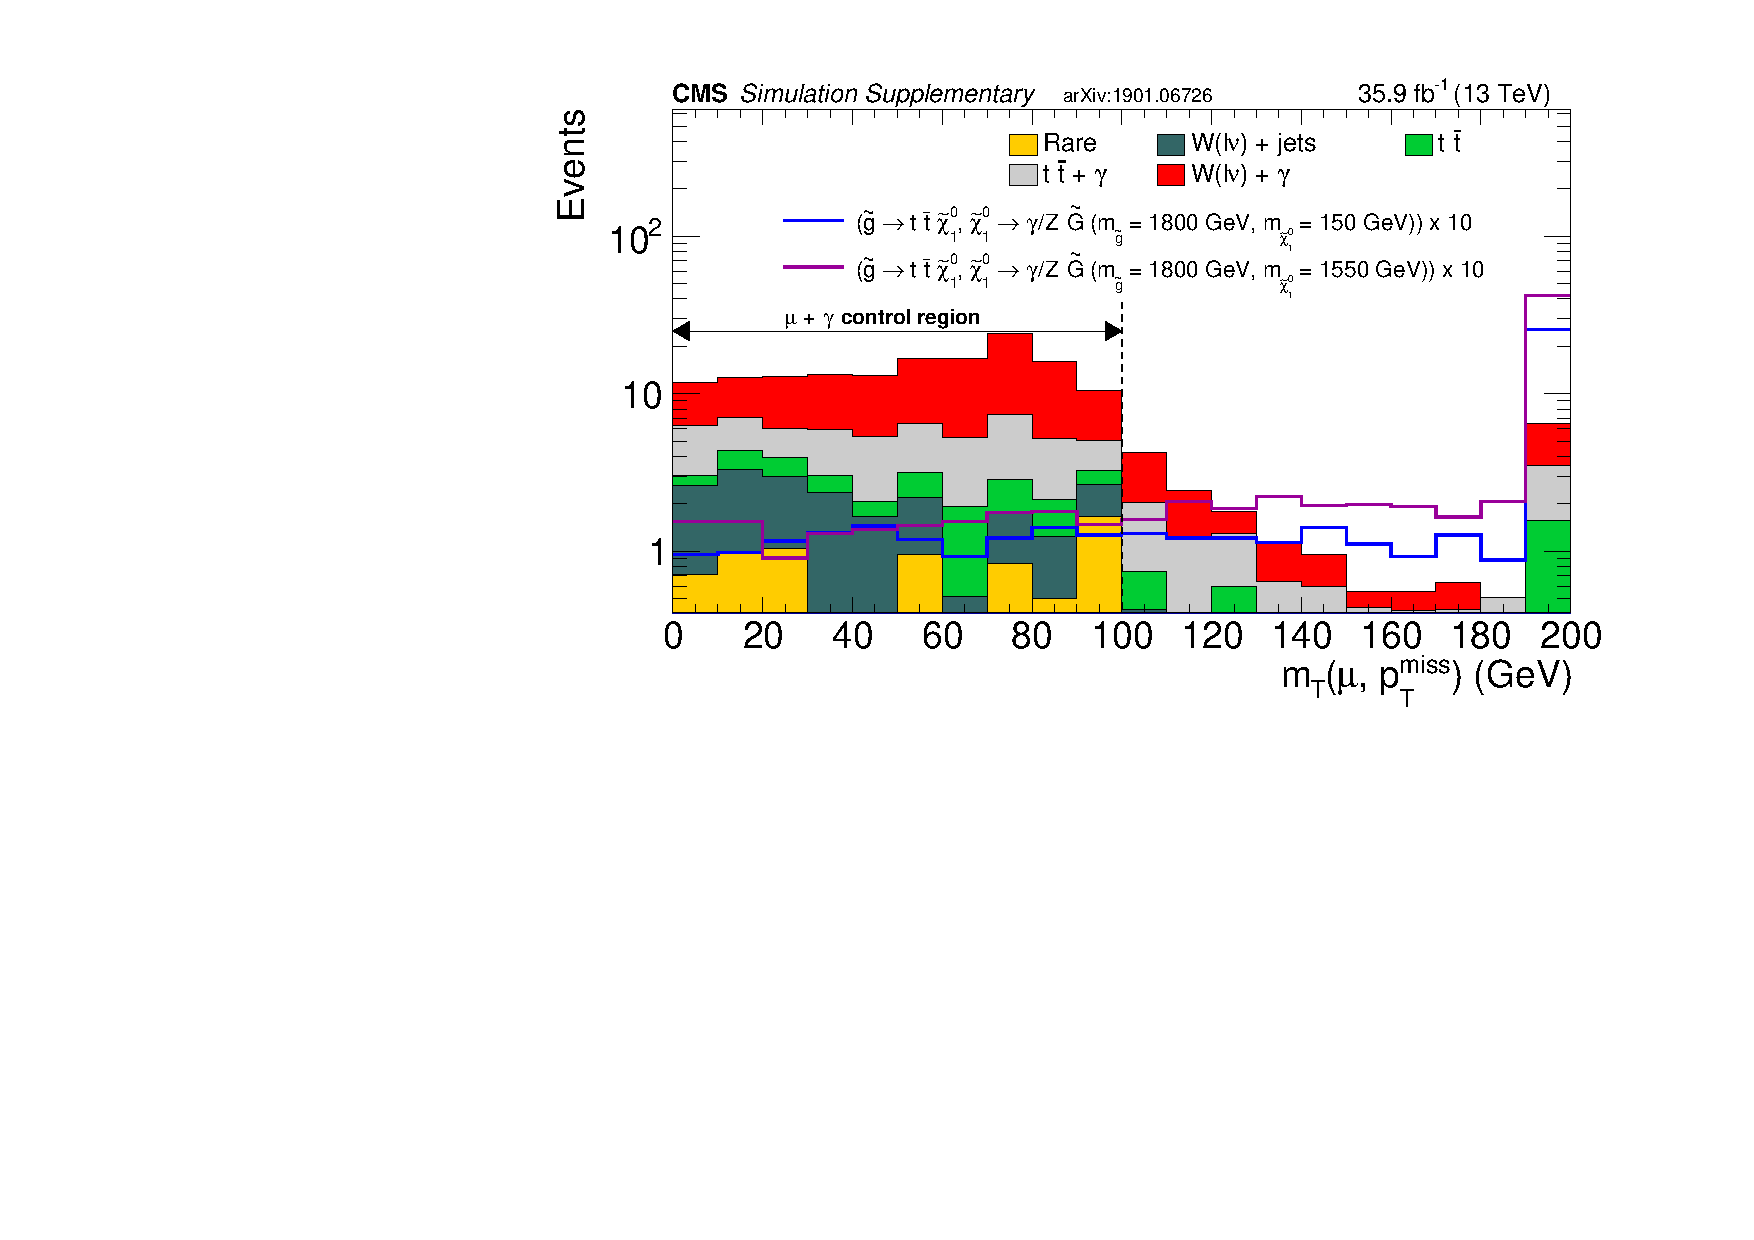
\includegraphics[width=0.8\linewidth]{../Figures/Chap3/anaPublic/supp_Sim_MuGammaCS_mT_T5ttttZG}
\captionsetup{width=.9\linewidth}
\caption[$m_T$ distribution for $\mu\gamma$ control region]{The transverse mass, $m_{T}$ distribution for $\mu\gamma$ events. Standard model processes are shown as filled histograms, representative signals of T5ttttZG model are shown as solid lines, and the signal is scaled up by a factor of 10 for better visualization.}
\label{fig:supp_Sim_MuGammaCS_mT_T5ttttZG}
\end{figure}

All other selections for the control region, isolated track vetos, \ST, \ptmiss, \nj,
and $\dphi$ are the same as the signal region. 
The control region events are triggered using the same triggers as the signal region
and the same trigger efficiency correction/efficiencies are applied.  

The method relies on weighting single lepton events. Event weights are derived
from simulations for electron and muon control samples separately.  The event 
weights are derived according to,
\begin{equation} \label{eq1}
\begin{split}
N_{lost-\ell}^{pred} & = N_{\ell}^{data}(\ptmiss,\nj,\nb) \cdot T^{\text{MC}}(\ptmiss,\nj,\nb)\\
\mathrm{where\ } T^{\text{MC}}(\ptmiss,\nj,\nb) & = N^{\text{MC}}_{lost-\ell}(\ptmiss,\nj,\nb) / N^{\text{MC}}_{\ell}(\ptmiss,\nj,\nb)
\end{split}
\end{equation}
$N_{\ell}^{data}$ and $T^{\text{MC}}$ are the observed yields in the control region
and the simulation-derived event weight for a corresponding search region.
For the muon ($\ell=\mu$) transfer factors, we include events with zero e,$\mu$, but at least one
hadronic-$\tau$ in the numerator of the transfer factor.

\begin{table}
\centering
\captionsetup{width=.9\linewidth}
\caption{Parameterization of transfer factors for lost-e and lost-$\mu+\tau_{\text{had}}$ events.}
\label{tab:lost_lepton_SF}
{\renewcommand{\arraystretch}{1.3}}% for the vertical padding
\begin{tabular}{c|c|c|c|c|c}
\hline
                          &            & \multicolumn{4}{c}{Event weight} \\ \cline{3-6}
                          &            & \multicolumn{2}{c|}{High-\dphi}   &\multicolumn{2}{c}{Low-\dphi} \\ \cline{3-6}
$N_{\mathrm{jets}}^{\mathrm{b-jets}}$       & \ptmiss    & Lost-e            & Lost-$\mu+\tau_{\text{had}}$ & Lost-e         & Lost-$\mu+\tau_{\text{had}}$ \\ \hline \hline
\multirow{2}{*}{$N_{2}^0$}& 100-150    & 0.55 $\pm$ 0.06 & 1.05 $\pm$ 0.07  & 0.23 $\pm$ 0.04 & 0.75 $\pm$ 0.10 \\ \cline{2-6}
                          & $\geq 150$ & 0.42 $\pm$ 0.04 & 0.84 $\pm$ 0.06  & 0.24 $\pm$ 0.04 & 0.66 $\pm$ 0.10 \\ \cline{1-6}
\multirow{2}{*}{$N_{3}^0$}& 100-150    & 0.30 $\pm$ 0.04 & 0.81 $\pm$ 0.06  & 0.20 $\pm$ 0.04 & 0.59 $\pm$ 0.12 \\ \cline{2-6}
                          & $\geq 150$ & 0.30 $\pm$ 0.04 & 0.67 $\pm$ 0.06  & 0.21 $\pm$ 0.04 & 0.54 $\pm$ 0.13 \\ \cline{1-6}
\multirow{2}{*}{$N_{4}^0$}& 100-150    & 0.29 $\pm$ 0.06 & 0.62 $\pm$ 0.10  & 0.26 $\pm$ 0.08 & 0.43 $\pm$ 0.12 \\ \cline{2-6}
						  & $\geq 150$ & 0.64 $\pm$ 0.06 & 1.23 $\pm$ 0.08  & 0.20 $\pm$ 0.04 & 0.67 $\pm$ 0.07 \\ \cline{1-6}
\multirow{2}{*}{$N_{5-6}^0$}& 100-150    & 0.30 $\pm$ 0.02 & 0.97 $\pm$ 0.05  & 0.16 $\pm$ 0.03 & 0.60 $\pm$ 0.07 \\ \cline{2-6}
                            & $\geq 150$ & 0.36 $\pm$ 0.03 & 0.79 $\pm$ 0.05  & 0.11 $\pm$ 0.02 & 0.43 $\pm$ 0.05 \\ \cline{1-6}
\multirow{2}{*}{$N_{\geq 6}^0$}& 100-150    & 0.25 $\pm$ 0.03 & 0.64 $\pm$ 0.04  & 0.17 $\pm$ 0.03 & 0.54 $\pm$ 0.07 \\ \cline{2-6}
                               & $\geq 150$ & 0.33 $\pm$ 0.08 & 0.73 $\pm$ 0.10  & 0.17 $\pm$ 0.05 & 0.59 $\pm$ 0.20 \\ \hline
\multirow{2}{*}{$N_{2-4}^{\geq 1}$}& 100-150 & 0.51 $\pm$ 0.05 & 0.87 $\pm$ 0.09  & 0.43 $\pm$ 0.06 & 0.98 $\pm$ 0.18 \\ \cline{2-6}
                          & $\geq 150$ & 0.39 $\pm$ 0.04 & 0.70 $\pm$ 0.07  & 0.21 $\pm$ 0.06 & 0.81 $\pm$ 0.15 \\ \cline{1-6}
\multirow{2}{*}{$N_{5-6}^{\geq 1}$}& 100-150    & 0.44 $\pm$ 0.08 & 0.64 $\pm$ 0.09  & 0.27 $\pm$ 0.09 & 0.45 $\pm$ 0.17 \\ \cline{2-6}
						  & $\geq 150$ & 0.57 $\pm$ 0.05 & 1.11 $\pm$ 0.10  & 0.27 $\pm$ 0.04 & 0.68 $\pm$ 0.10 \\ \cline{1-6}
\multirow{2}{*}{$N_{\geq 6}^{\geq 1}$} & 100-150    & 0.35 $\pm$ 0.04 & 0.79 $\pm$ 0.07  & 0.25 $\pm$ 0.04 & 0.54 $\pm$ 0.07 \\ \cline{2-6}
                          & $\geq 150$ & 0.36 $\pm$ 0.06 & 0.67 $\pm$ 0.10  & 0.25 $\pm$ 0.06 & 0.53 $\pm$ 0.10 \\\hline
\end{tabular}
\end{table}

Table~\ref{tab:lost_lepton_SF} shows the event weights for the two lost-lepton control regions.
These weights are typically 0.5 (0.75) for the e ($\mu$) control regions. 

To test the paremeterization of the event weights, the lost lepton method is evaluated 
on simulated data.  Figure~\ref{fig:lost_lepton_closure} shows comparisons of the predicted event yield
in each of the search regions and the true event yield from simulation for the electron
and $\mu+\tauh$ events.  The event weight parameterization is found to 
predict the true event yield for each of the search regions with the largest observed
deviation corresponding to a 30\% discrepancy, which is consistent with expectations
from statistical fluctuation only. 
The uncertainty on the event weights from limited MC statistics is propagated to the final predictions.
Any non-closure seen in the tighter \ptmiss region will be covered by the control sample statistical uncertainty in data.
%\textcolor{red}{Add 1D pull ../Figures/Chap3 for closure.}.

To model the uncertainty on the prediction due to limited statistics from the single 
lepton control regions, each prediction will have a prior distribution modeled by
a gamma distribution that uses the observed control region statistics and the average 
transfer factor.  The average transfer factor is defined to be the prediction 
divided by the raw observed control region event yield.  In bins where there are
no events observed, the average transfer factor is computed based on MC events 
yields.  

\begin{figure}
\centering
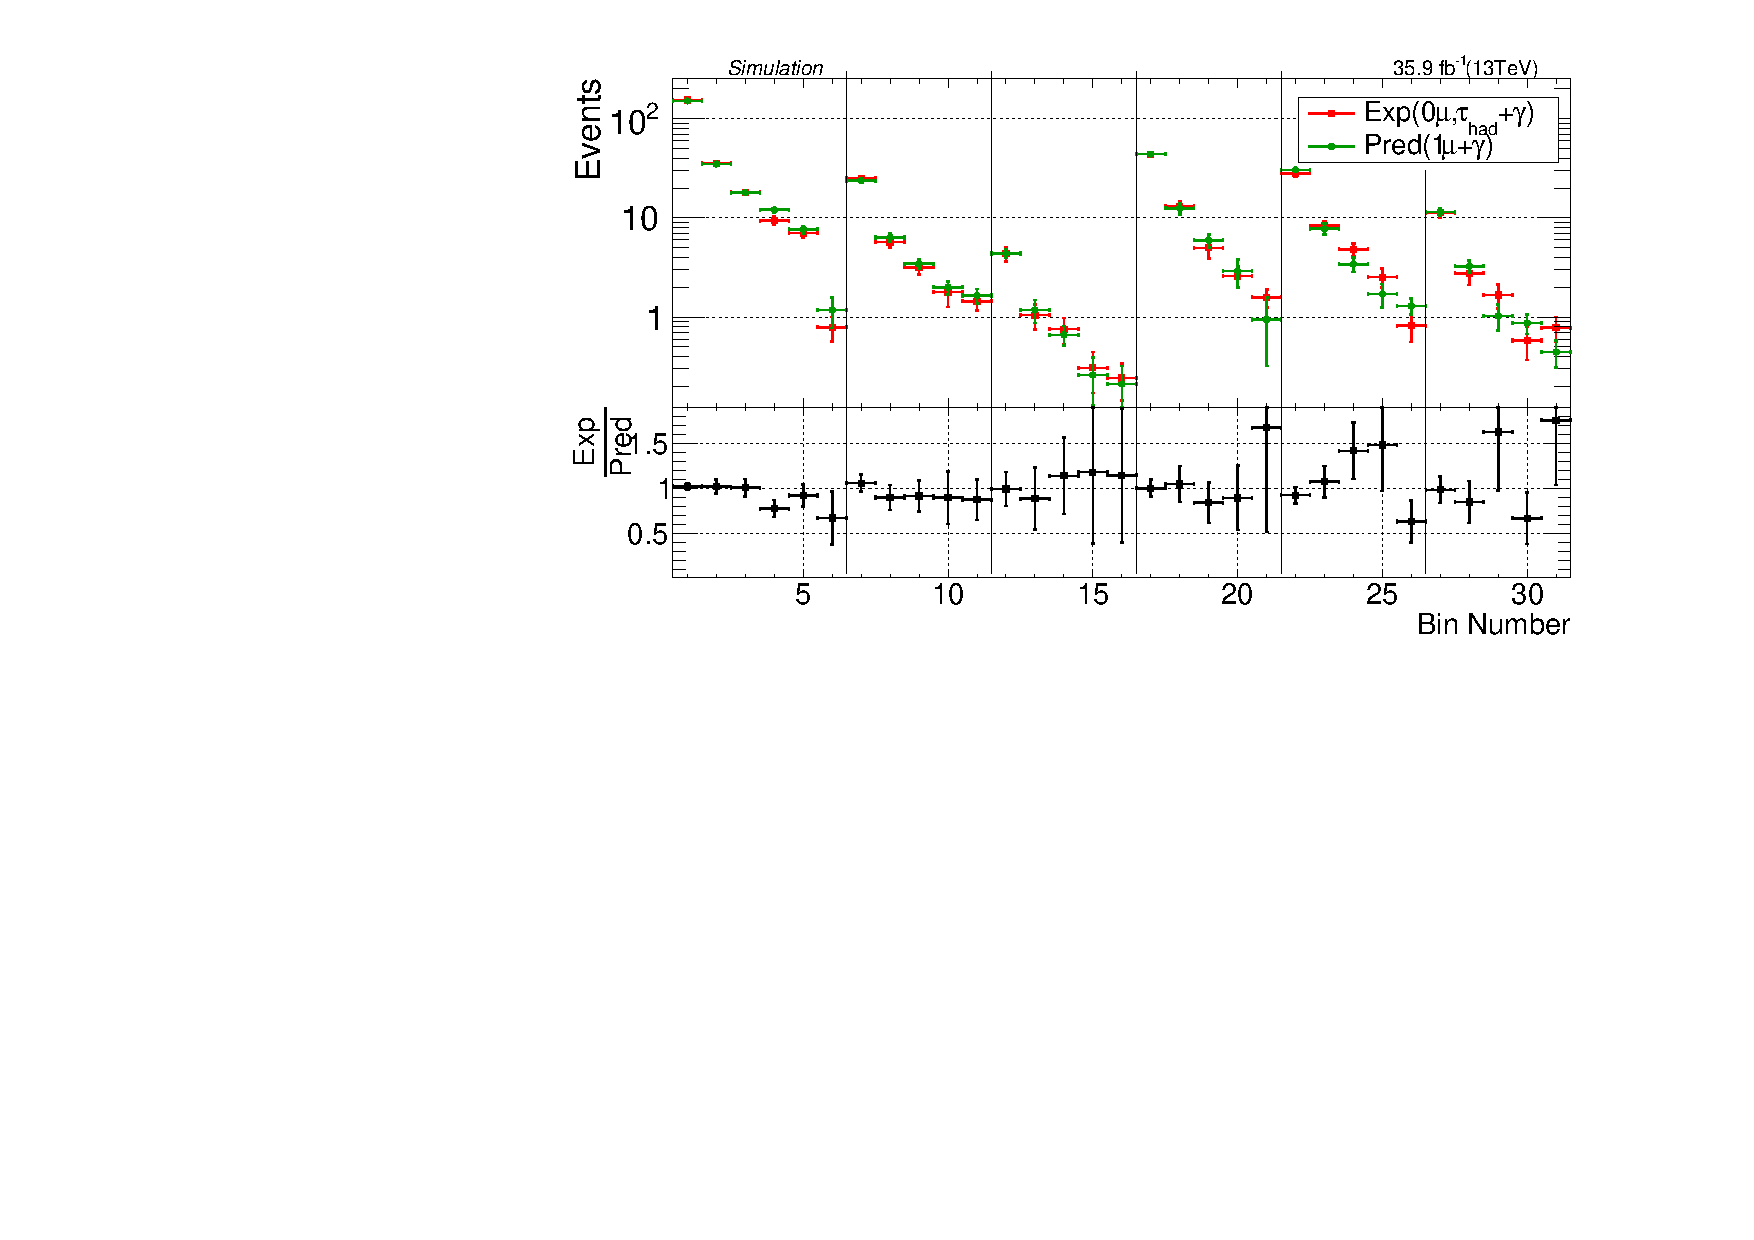
\includegraphics[width=0.48\linewidth]{../Figures/Chap3/SUSY_Photon_MET_JbJ_18Aug17/LostMu_Closure/AllSBins_v7_Mu0AllSBins_v7_Mu1.pdf}
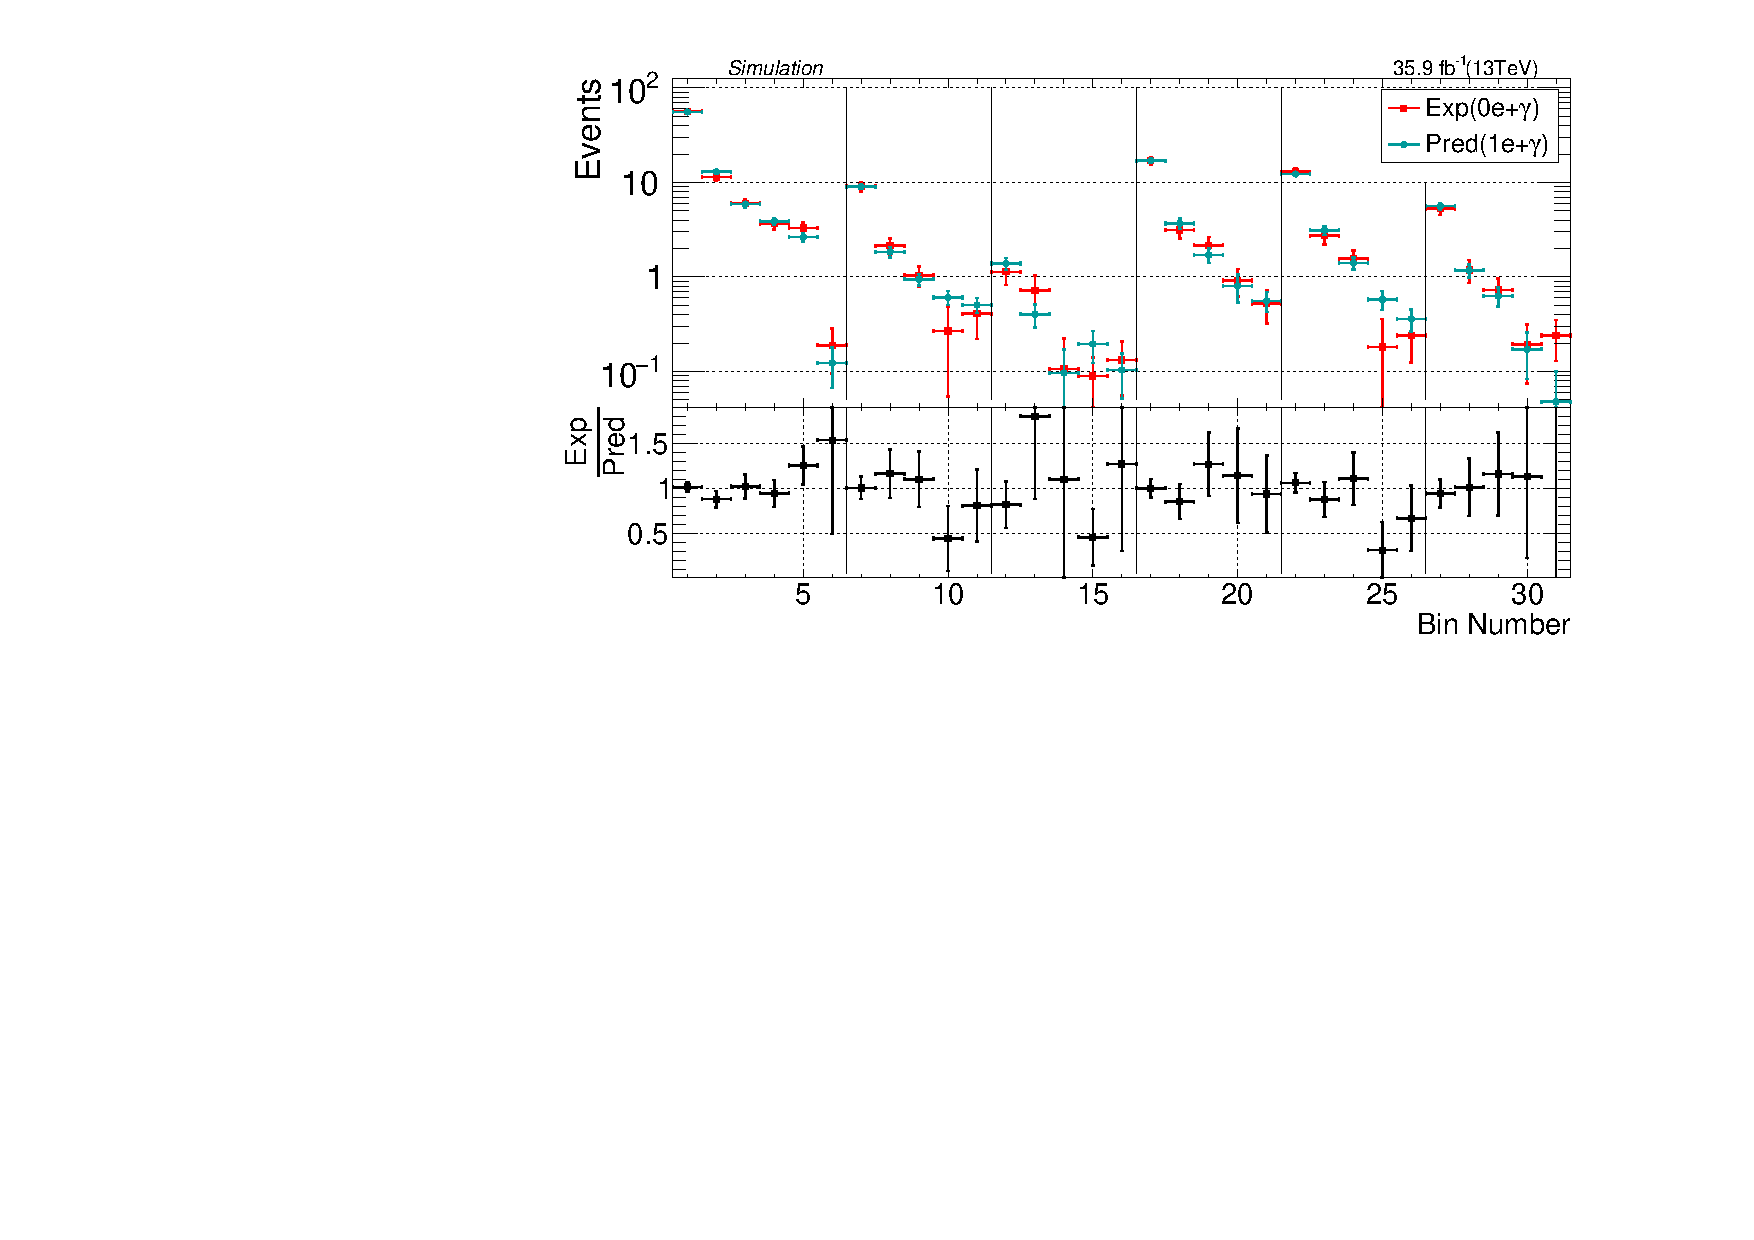
\includegraphics[width=0.48\linewidth]{../Figures/Chap3/SUSY_Photon_MET_JbJ_18Aug17/LostEle_Closure/AllSBins_v7_Ele0AllSBins_v7_Ele1.pdf}
\captionsetup{width=.9\linewidth}
\caption{Expected closure of lost electron (left) and lost $\mu+\tauh$ (right) predictions
where simulated event yields are treated like data.}
\label{fig:lost_lepton_closure}
\end{figure}

Other sources of systematic uncertainty correspond to effects related to:
\begin{itemize}
  \item lepton scale factors
  \item b-tagging scale factors
  \item PDF and scale uncertainties
  \item modeling of \mt in simulations
  \item modeling of colinear photons 
\end{itemize}

The PDF and scale uncertainties are studied by varying the MC weights according
to 101 and 9 weight sets respectively.  For each variation the average transfer factor for
all signal regions combined is computed.  
The maximum variation of the lost $\mu+\tauh$
average transfer factor is found to be 1.3\% and 0.7\% for the PDF and scale variations, 
respectively.  
The maximum variation of the lost $mu$ average TF is found to be 1.3\% and 0.7\% for the PDF and scale variations respectively.
For the lost-e, 4.8\% and 1.0\% variations were found in TF because of the PDF and scale variations, respectively.
The maximum variation of these alternative weights is added as a systematic 
uncertainty on the lost-lepton and $\tauh$ prediction. A single nuisnace parameter
is used to model this uncertainty, correlating all signal regions and correlating
the effect of PDF and scale uncertainties for both lost-e and lost-$\mu+\tauh$
predictions. 

The effect of JEC uncertainties are studied by varying both jet \pt and \ptmiss.
This variation can cause events 
to migrate below the minimum \ptmiss or \ST thresholds, or above the maximum
\mt threshold for single lepton events.  No trends are observed versus 
the various signal region.  There is a 2\% (0.6\%) effect on the lost-e (lost-$\mu+\tauh$)
transfer factor, averaged over all signal regions.  The 2\% effect for the lost-e 
prediction is applied as a systematic uncertainty.  The effect on the lost-$\mu+\tauh$
prediction is neglected.
The same correlation model as used for the PDF and scale uncertainties is applied
for the JEC uncertainty systematic.  

The modeling of the \mt distribution is potentially effected by generator
level cuts in MC samples, but this effect is found to be
less than 1\% and is neglected.

The effect of uncertainties on the lepton scale factors are propagated
to the lost-e and lost-$\mu+\tauh$ transfer factors.  These are found to have
a 2\% effect, which is assumed to be correlated among common \ptmiss bins.  

Finally the effect of b-tagging scale factor uncertainties was checked.  
It was found to have $<1\%$ effect on the lost-lepton transfer factors
and is neglected. 

Comparisons between simulation and data for single lepton events show
a systematic mismodeling of events with small angle between the e/$\mu$
and the photon.  This is due to generator level cuts on the angle between
photons and partons, in Madgraph W/$t\bar{t}+\gamma$ samples, of $\Delta R<0.5$,
which is not well modeled by pythia W/$t\bar{t}$+jets samples. Figure~\ref{fig:lost_ell_dR_dist}
shows the $\Delta R(e,\gamma)$ and $\Delta R(\mu,\gamma)$ distributions.  
The region $\Delta R(e,\gamma)<0.2$ is excluded due to the photon/electron
isolation cuts. To assess the effect of the missing low $\Delta R$
phase space, the average transfer factor is derived for events with 
$\Delta R>0.5$ and compared to the average transfer factor computed 
with all events.  The effect is found to be a 12\%
effect on the lost-e transfer factor and $<1\%$ on the 
lost-$\mu+\tauh$ transfer factor.  Since no trends are found versus various 
signal regions, a flat 12\% uncertainty is applied
to lost-e prediction.  No systematic uncertainty is applied to
the lost-$\mu+\tauh$ prediction.

\begin{figure}
\centering
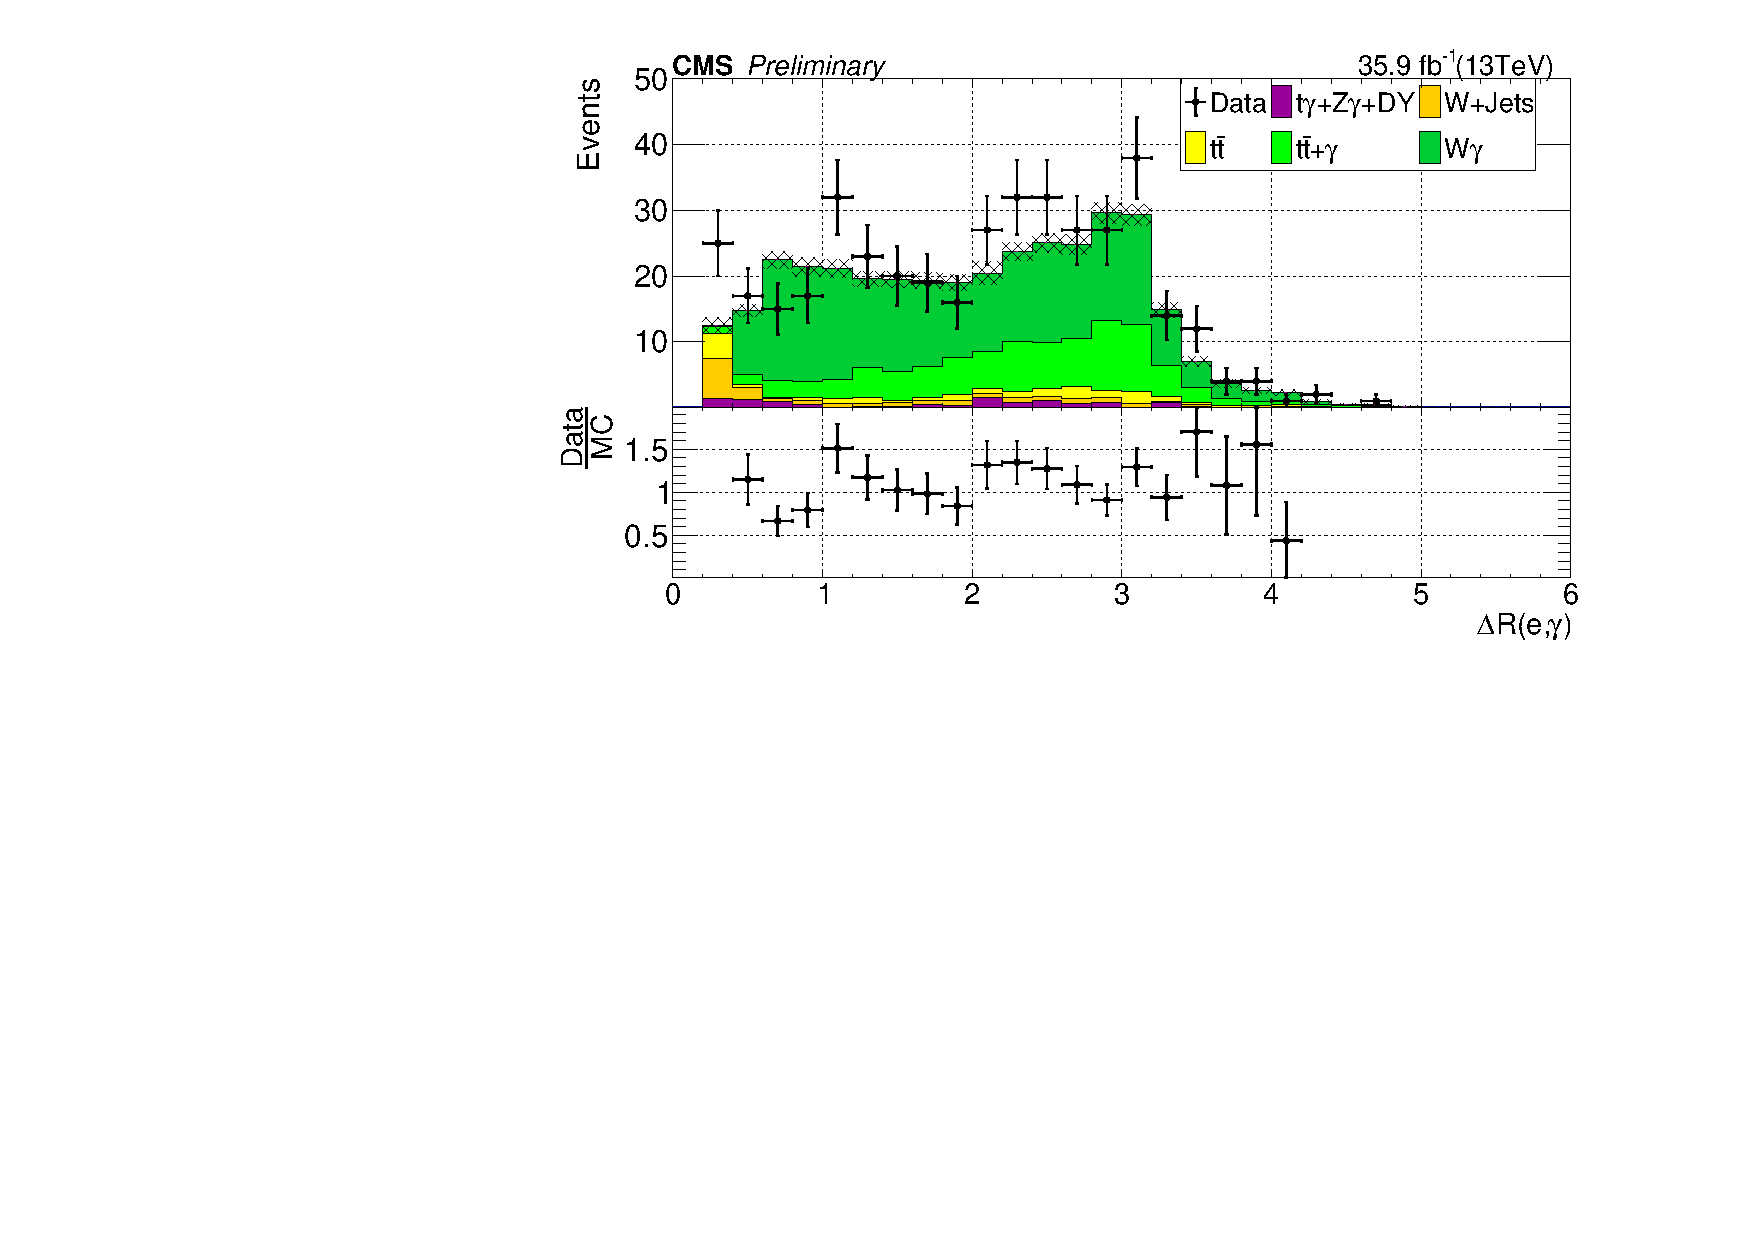
\includegraphics[width=0.48\linewidth]{../Figures/Chap3/lost_lepton/lostElectronDeltaR.pdf}
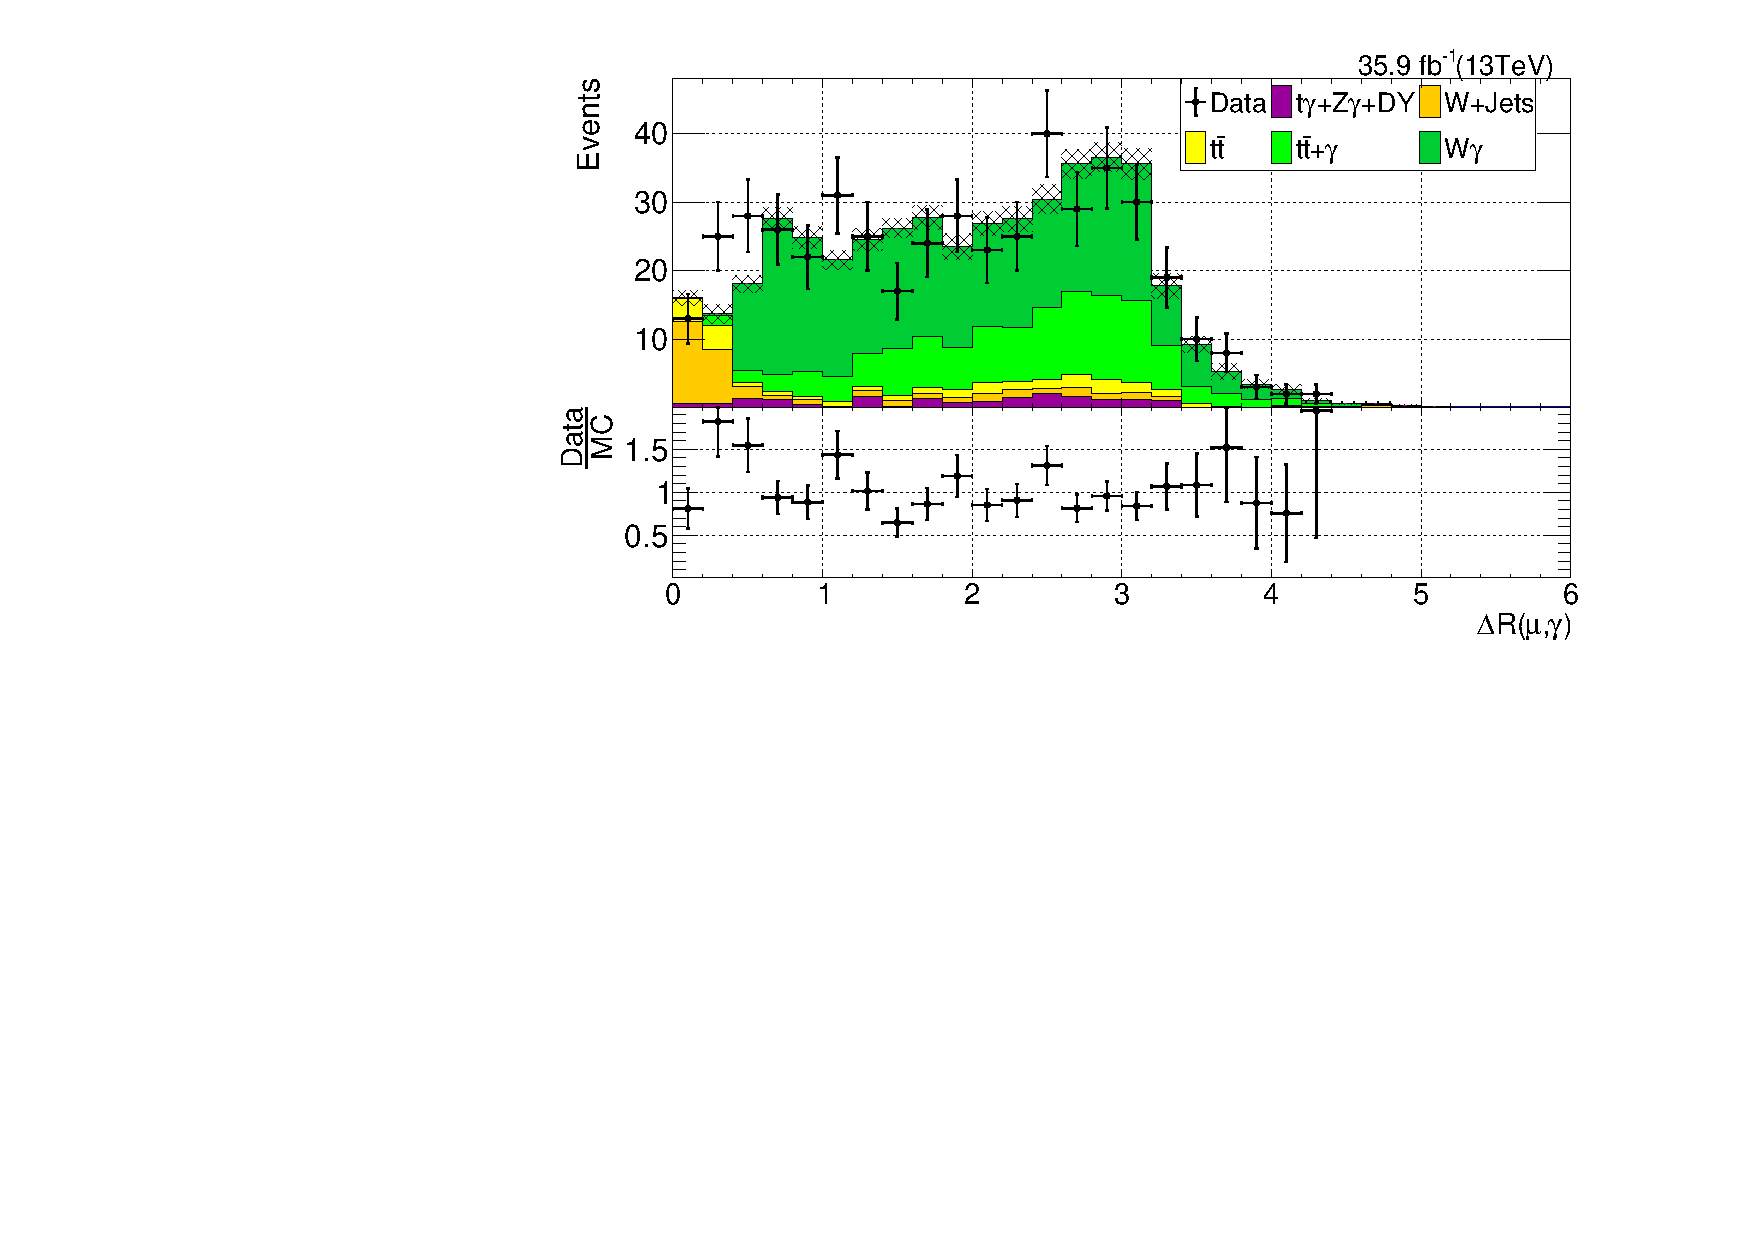
\includegraphics[width=0.48\linewidth]{../Figures/Chap3/lost_lepton/lostMuonDeltaR.pdf}
\captionsetup{width=.9\linewidth}
\caption{Distribution of $\Delta R(\ell,\gamma)$ for single
electron (left) and single muon (right) events.}
\label{fig:lost_ell_dR_dist}
\end{figure}

The observed event yields and the corresponding predictions are shown in Table~\ref{tab:lostLeptonPredictions} (for high \dphi) and Table~\ref{tab:lostLeptonPredictions_LDP} (for low \dphi) of appendix \ref{AppendixB}. 
Comparisons of the observed yields and expected MC yields for the $e+\gamma$ and $\mu+\gamma$ control 
regions in Figures~\ref{fig:lost_mu_CR_dist} and~\ref{fig:lost_e_CR_dist} of appendix \ref{AppendixC}.


\subsection{Estimation of events with electrons faking photons}

The fake-rate estimation predicts the expected rate from $W(e\nu)$ 
events where the electron fakes a photon.  The method relies on
computing an $e\rightarrow\gamma$ fake rate, derived from a mixture
of simulation and data, and applying the fake rate as an event weight
to the single electron control region, in which we veto events with
a photon.  

The kinematic selection for the single electron control region is exactly the 
same as the single photon control region except that we require exactly 
zero photons, exactly one electron with tight ID criteria, and use the tight electron
4-vector in place of the photon 4-vector where relevant. 

The crux of this method is the derivation of the fake rate.  The fake
rate in a given region of phase space is defined to be the ratio of events 
with photons and no electron with respect 
to events with exactly one tight electron and zero photons.  The 
fake rate will be derived using simulated W/$t\bar{t}$ events.  
However, due to MC modeling of various nuisances relevant to electron
reconstruction, an overall difference is to be expected between 
data and MC fake-rates.  To correct for this, we will also 
measure the fake-rate in data and MC using DY events with a 
tag-and-probe (T\&P) method.  These T\&P measurements will be 
used to correct the fake rates derived on W/$t\bar{t}$ simulations.

The overall prediction is then given by:
\begin{equation} \label{eqn:fake_pred}
  N_{e\rightarrow\gamma} = N_{e}^{data} \cdot f^{tt,W} \cdot \beta^{data/MC} \cdot \frac{\epsilon^{trig}_{SR}}{\epsilon^{trig}_{CR}},
\end{equation}
where $f^{tt,W}$ is the fake-rate derived from W/$t\bar{t}$ simulation, 
$\beta$ represents the T\&P corrections factors, and $\epsilon$ represents 
the measured trigger efficiency.

There are two important paramterizations, namely, $f^{tt,W}$ and $\beta$.  

\subsubsection{Fake-rate parameterization}

The fake rate is parameterized as a function of local metrics relevant to electron reconstruction;
the electron \pt and the charged track multiplicity, $Q_{mult}$ around the electron 
are found to give the best closure on MC.  The metric $Q_{mult}$ 
is defined to be the sum of charged PF candidates with the jet 
matched, $\dR<0.3$, to the electron. Since we require electrons have at least
$\pt>100~\gev$, the jet clustering algorithm almost always clusters
the electron into an AK4 jet.  On the rare occasions that there is 
no matched jet, the event is rejected.  The distribution of $Q_{mult}$
is shown in Figure~\ref{fig:qMultDist} for DY, W+jets, and $t\bar{t}$ events. 

\begin{figure}[h!]
\centering
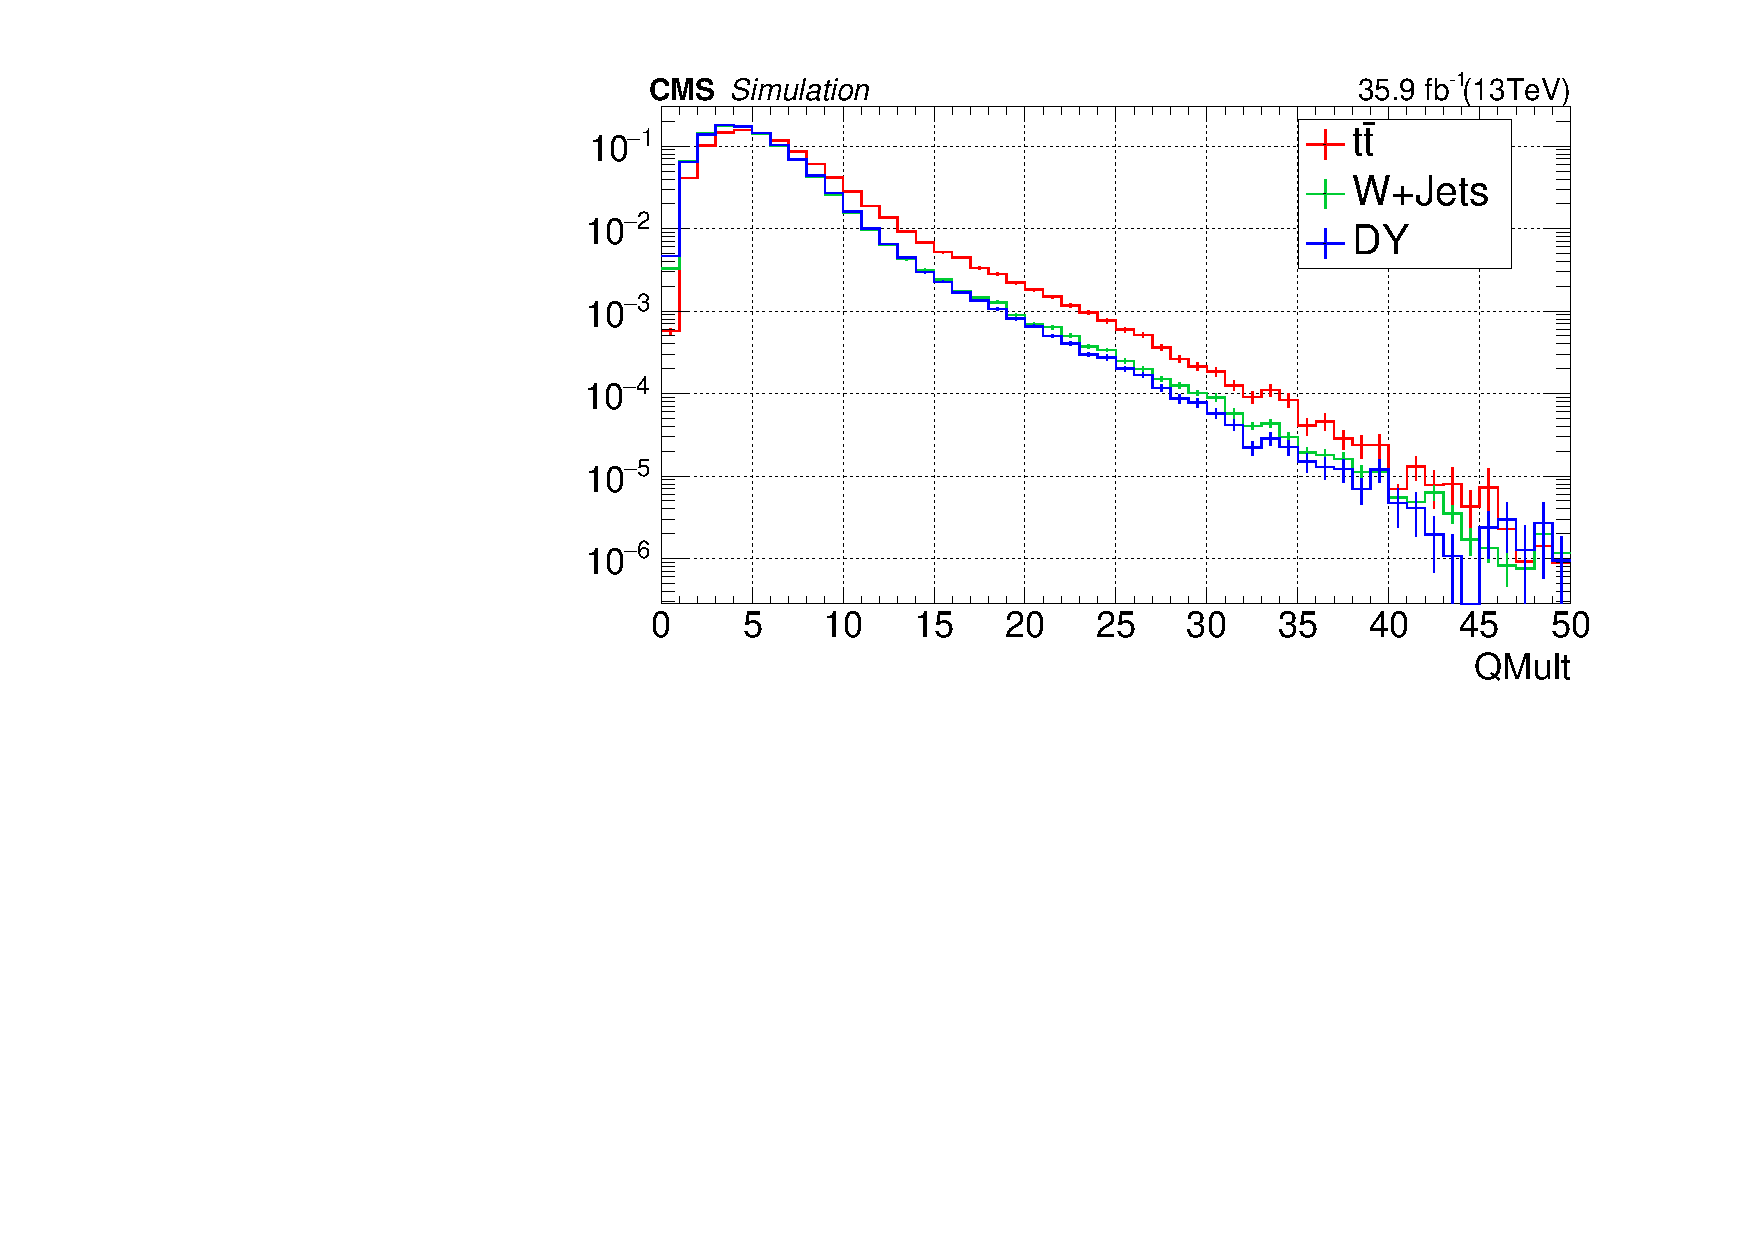
\includegraphics[width=0.48\linewidth]{../Figures/Chap3/fake_rate_closure/QMult_eleJet_ttwDY.pdf}
\caption[$Q_{mult}$ distribution for DY, W+jets, and $t\bar{t}$]{$Q_{mult}$ distribution in a jet matched to the electron in 
DY, W+jets, and $t\bar{t}$ events. Each of these distribution are scaled to unit area.}
\label{fig:qMultDist}
\end{figure}

When deriving the fake-rate from simulation events are divided into
two categories, signal region (SR) events, and control region (CR) events.  Signal region events are 
those with zero electrons found and an EM objects matched, $\dR<0.2$, to a gen-level
electron. Control region events are those with 1 tight electron ($\pt>100~gev$), 
exactly zero photons, and $m_T(e,\ptmiss)<100~\gev$; the last requirement 
increases the purity of the control sample and avoids overlap with 
signal events.  After these selections are applied, the fake rate is then
defined as $f^{tt,W}=N_{SR}/N_{CR}$.  

Table~\ref{tab:fakeRateParam} shows the parameterization
of the fake rate that is used.   To validate this parameterization, the
fake rate method is applied to MC and the prediction is compared to the 
true yields from simulation.  Figure~\ref{fig:fakeRateClosure} show the comparison 
of the prediction (applying the fake rate parameterization to single 
electron MC events) and true yields; the agreement is found to be 
within 20\%.
                            

\begin{figure}[h!]                           
\centering
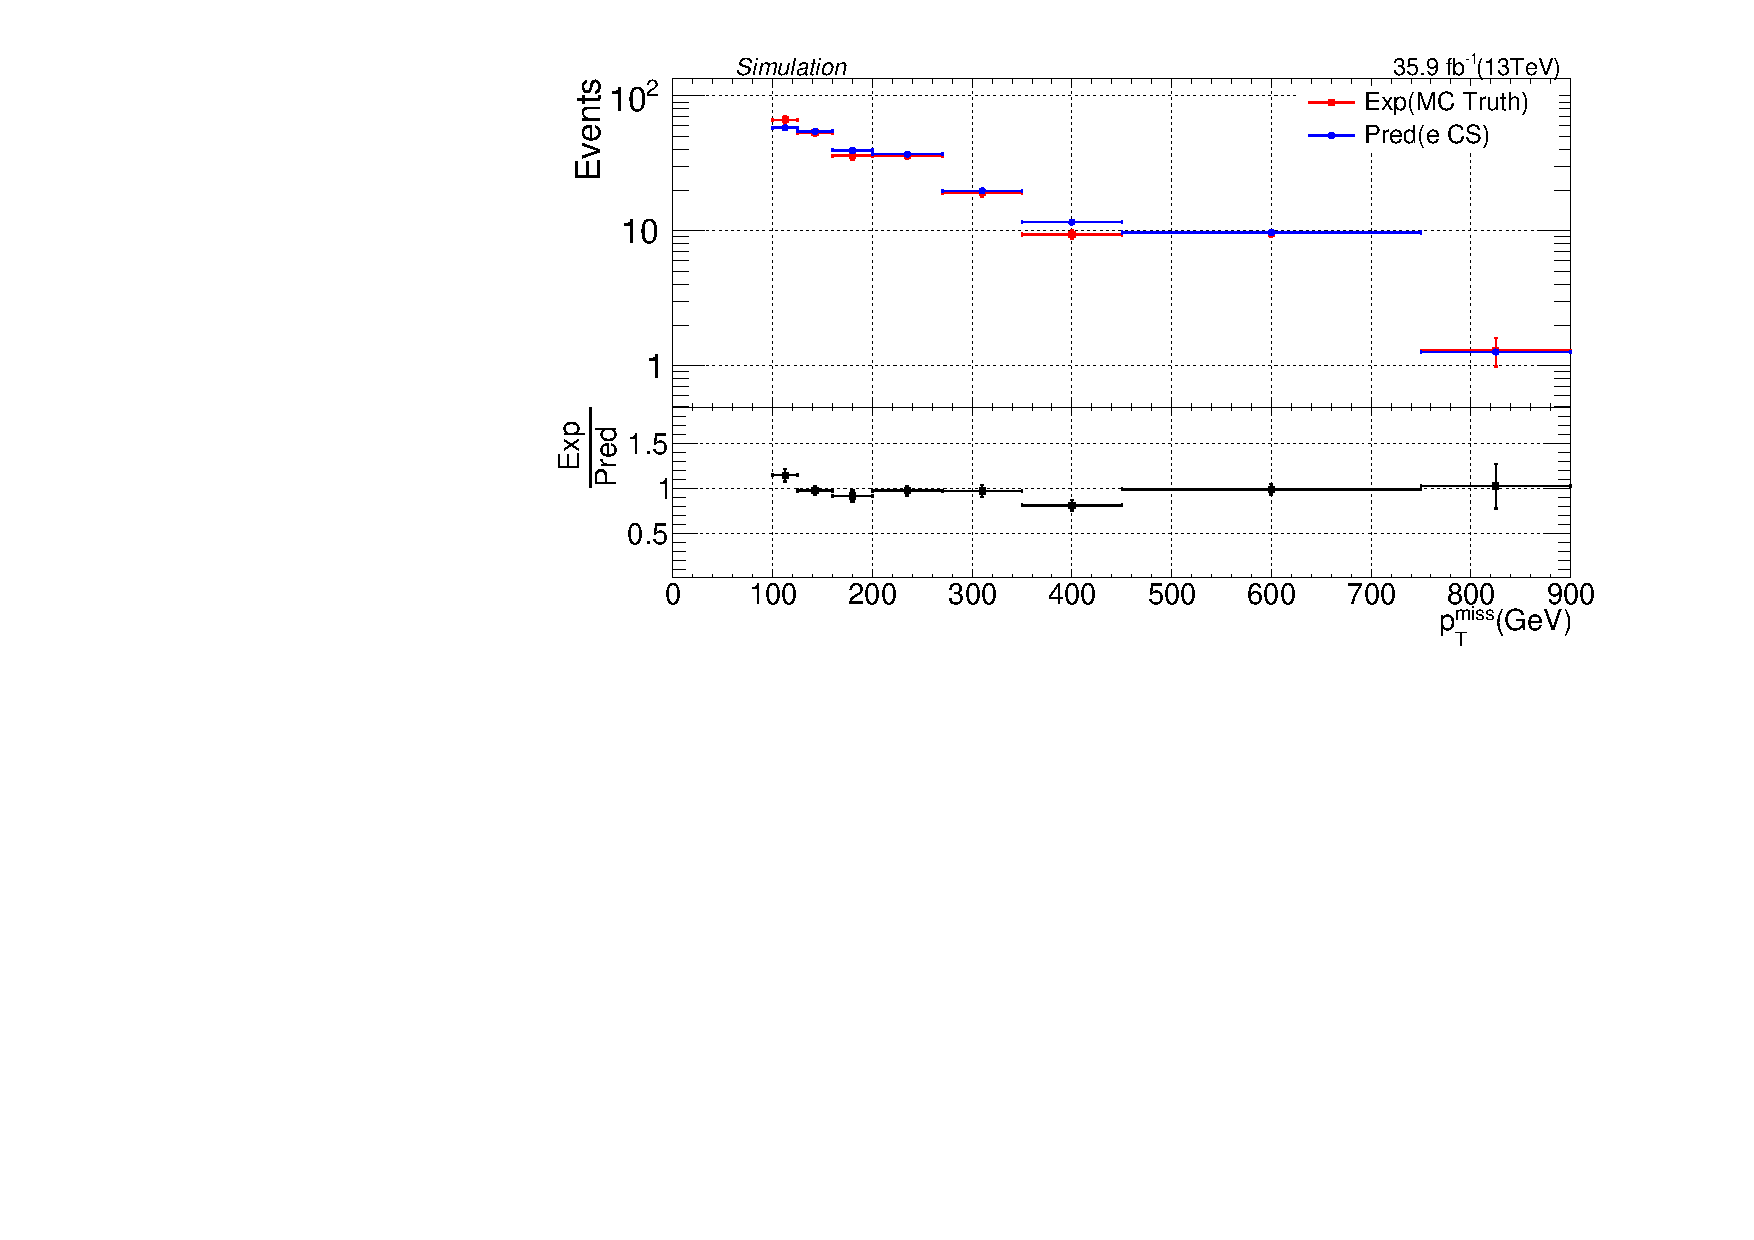
\includegraphics[width=0.48\linewidth]{../Figures/Chap3/fake_rate_closure/fakeRateClosure_met.pdf}
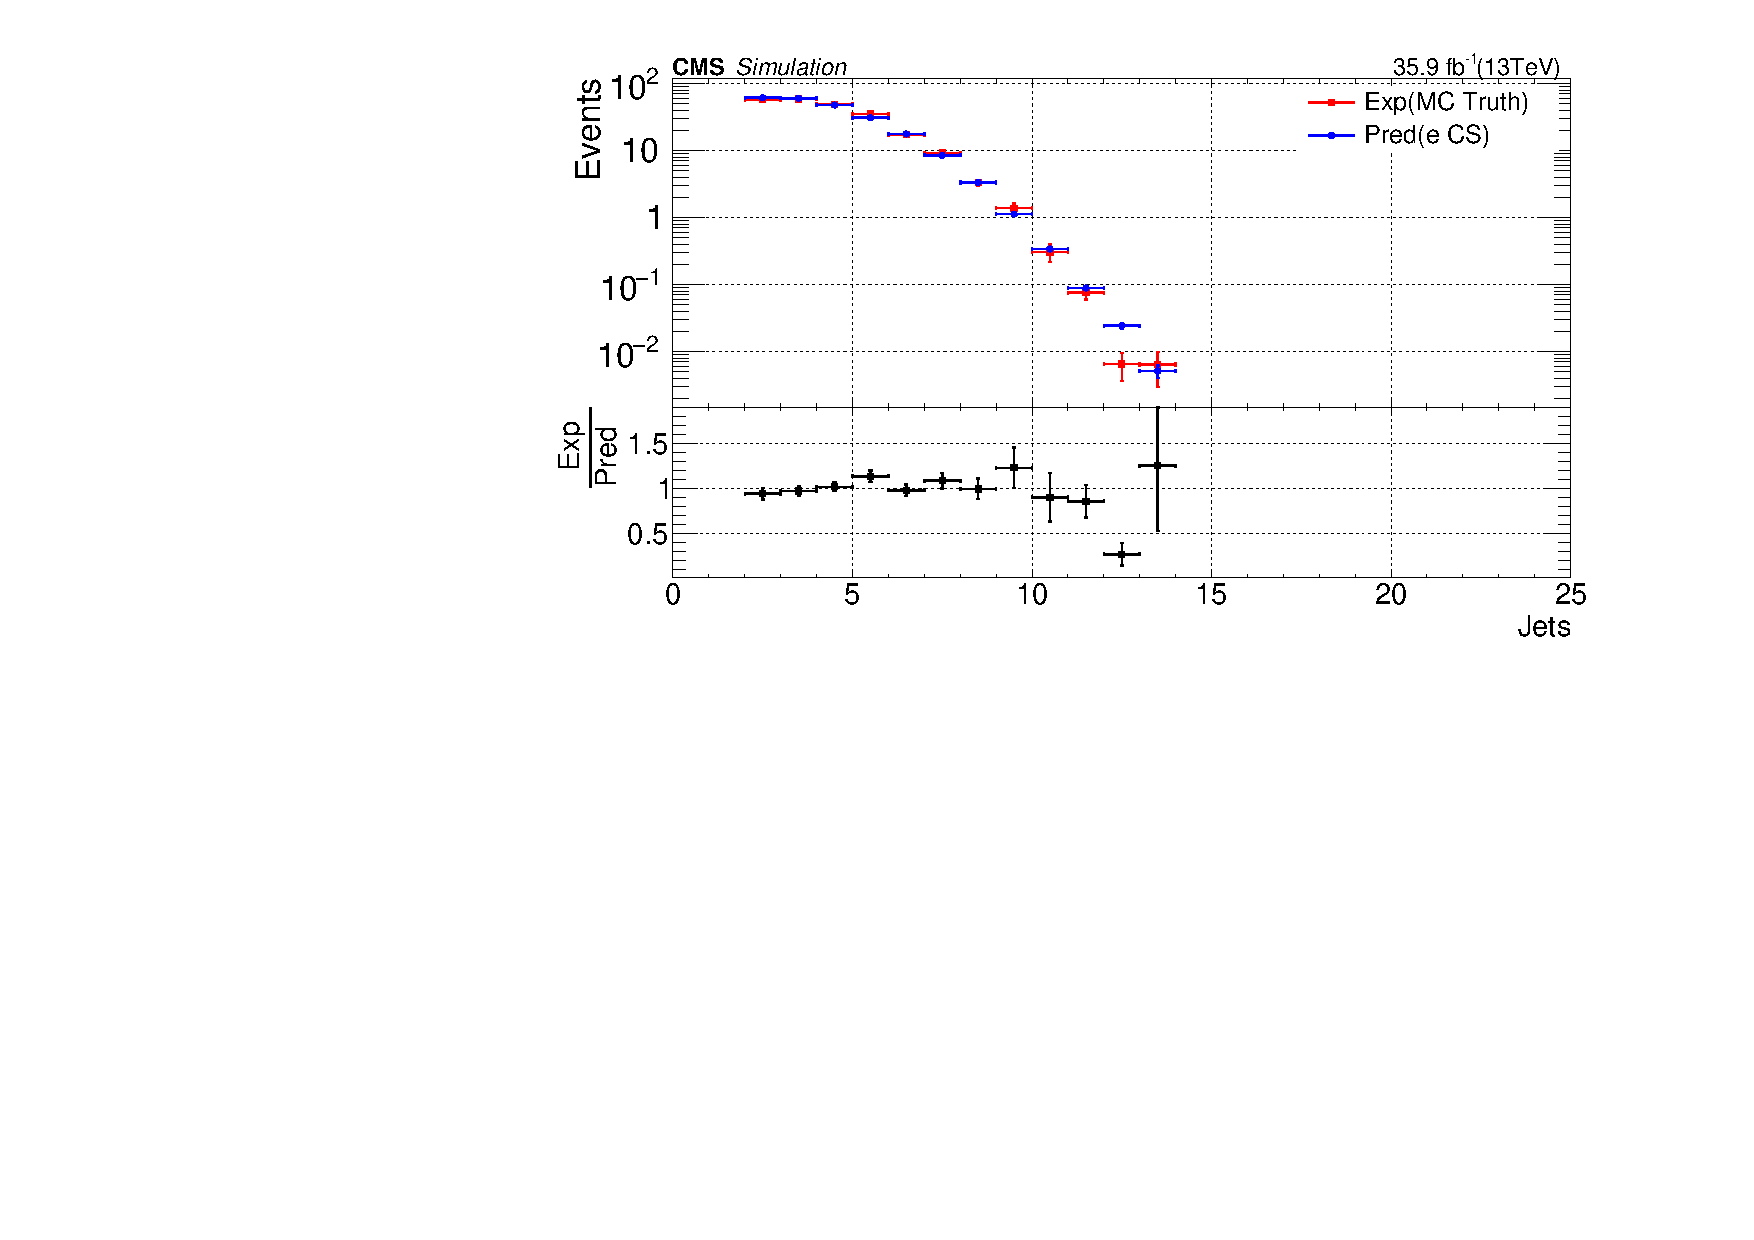
\includegraphics[width=0.48\linewidth]{../Figures/Chap3/fake_rate_closure/fakeRateClosure_njets.pdf}\\
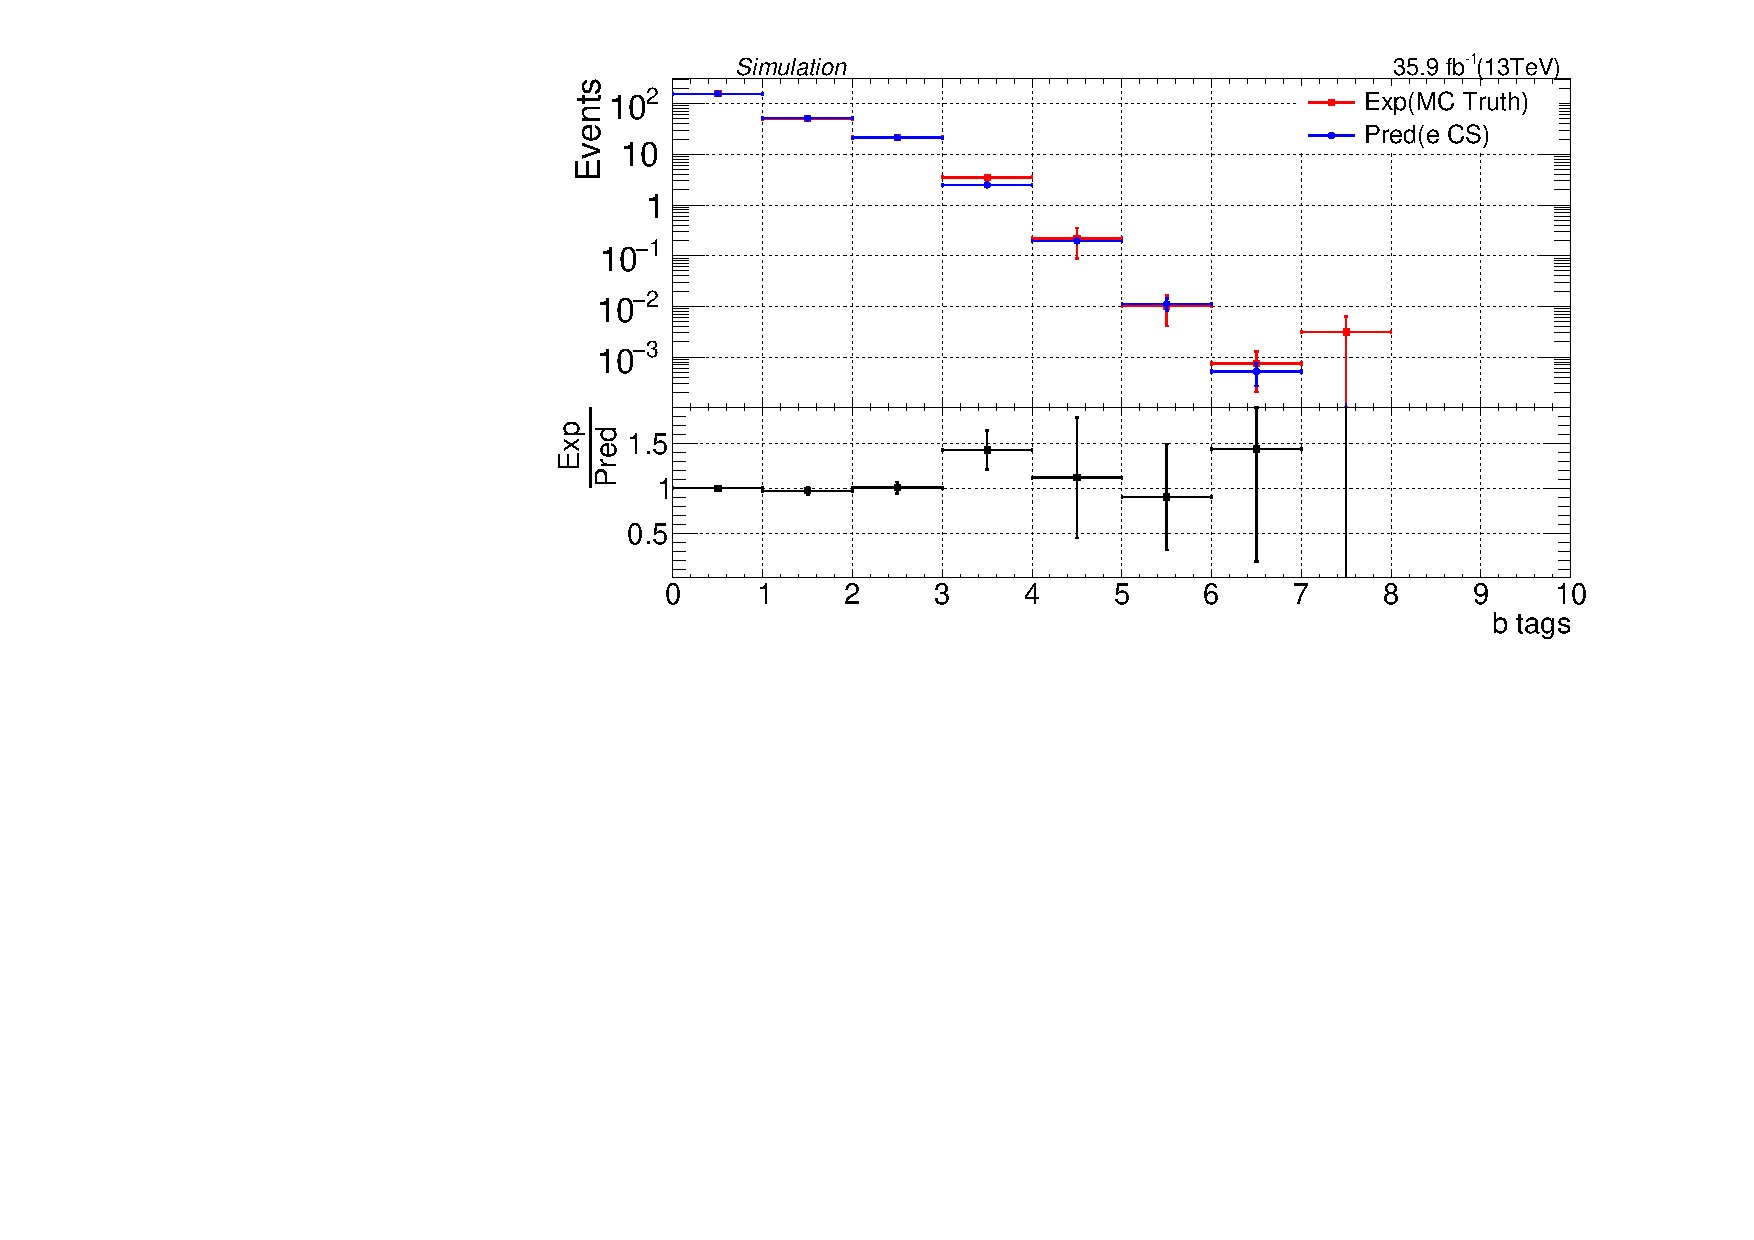
\includegraphics[width=0.48\linewidth]{../Figures/Chap3/fake_rate_closure/fakeRateClosure_btags.pdf}
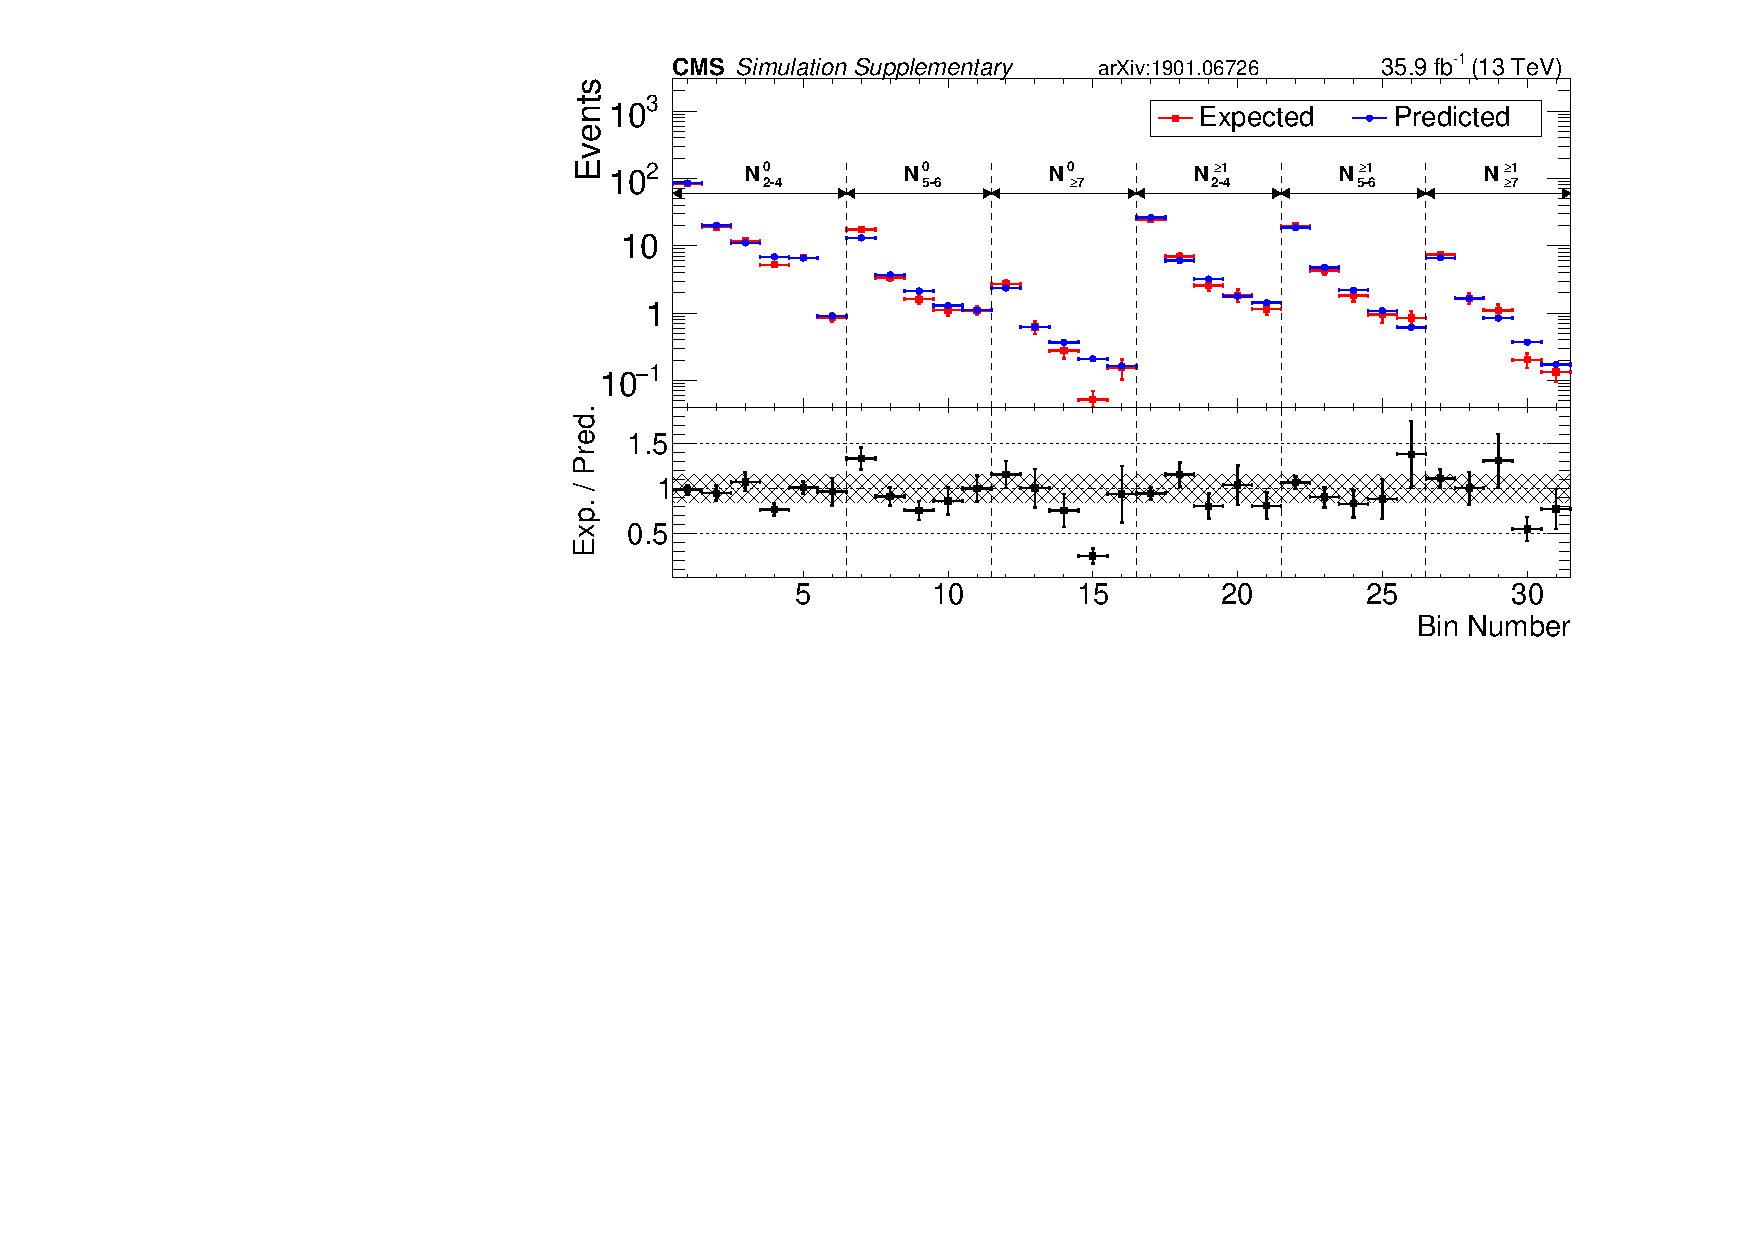
\includegraphics[width=0.48\linewidth]{../Figures/Chap3/anaPublic/fakerateClosure}
\captionsetup{width=.9\linewidth}
\caption[Fake rate closures]{Comparison of fake rate prediction using fake rate parameterization
and true MC yields using $W/t\bar{t}+(\gamma)$ simulations versus \ptmiss (top left), 
\nj (top right), \nb (bottom left) and search bins (bottom right). The hashed region in the lower panel 
of bottom right plot shows the total systematic uncertainty.}
\label{fig:fakeRateClosure}
\end{figure}

\subsubsection{Data/MC fake rate corrections}

The data/MC corrections for the fake rate are computed using a T\&P method on 
Drell-Yan events.  Z bosons are reconstructed using a tag object and a probe object.    
The tag object definition is one tight electron with $\pt>40~\gev$.  The probe
can either be one tight electron or one photon with $\pt>100~\gev$. Event selections
otherwise includes, $\nj\geq2$, $\ptmiss<100~\gev$, zero isolated tracks 
(not including the tag/probe objects), and \dR(tag, probe)$>0.2$. 
In the case where the probe satisfies the tag criteria, the tag is chosen
randomly and the event is counted twice. 

Once the photon and electron candidates are formed, the $m_{\ell\ell}$ distribution
is fit using a Briet-Wigner convoluted with a Gaussian to model the Z boson peak and
a polynomial to model the combinatorial background.  The fit is performed on 
both data and MC in regions of $Q_{mult}$, which is the variable for which 
the discrepancies between data and MC are found to be the largest. Table~\ref{tab:fakeRateCorrections}
shows the fitted fake rate in data and MC, and the corresponding correction
factor in each of the $Q_{mult}$ bins. Figure~\ref{fig:tpFits} shows the 
fit results for each of the fake rate measurements.

\begin{table}[h!]
\centering
\caption[Fake rate SFs]{Fake rate as measured by T\&P procedure on Drell-Yan events in data and MC.}
\label{tab:fakeRateCorrections}
\begin{tabular}{c|c|c|c}
\hline
$Q_{mult}$ & MC fake rate    & data fake rate  & scale factor \\ \hline\hline

0-1        & 0.014 $\pm$ 0.002    & 0.016 $\pm$ 0.003    & 1.17 $\pm$ 0.27  \\ \hline
$\geq$2    & 0.015 $\pm$ 0.001    & 0.018 $\pm$ 0.002    & 1.21 $\pm$ 0.16  \\ \hline
%2-3        & 0.014 $\pm$     & 0.018 $\pm$     & 1.28 $\pm$   \\ \hline
%4-5        & 0.013 $\pm$     & 0.016 $\pm$     & 1.26 $\pm$   \\ \hline
%6-7        & 0.014 $\pm$     & 0.019 $\pm$     & 1.34 $\pm$   \\ \hline
%$\geq$8    & 0.016 $\pm$     & 0.020 $\pm$     & 1.25 $\pm$   \\ \hline
\end{tabular}
\end{table}

\begin{figure}[h!]
\centering
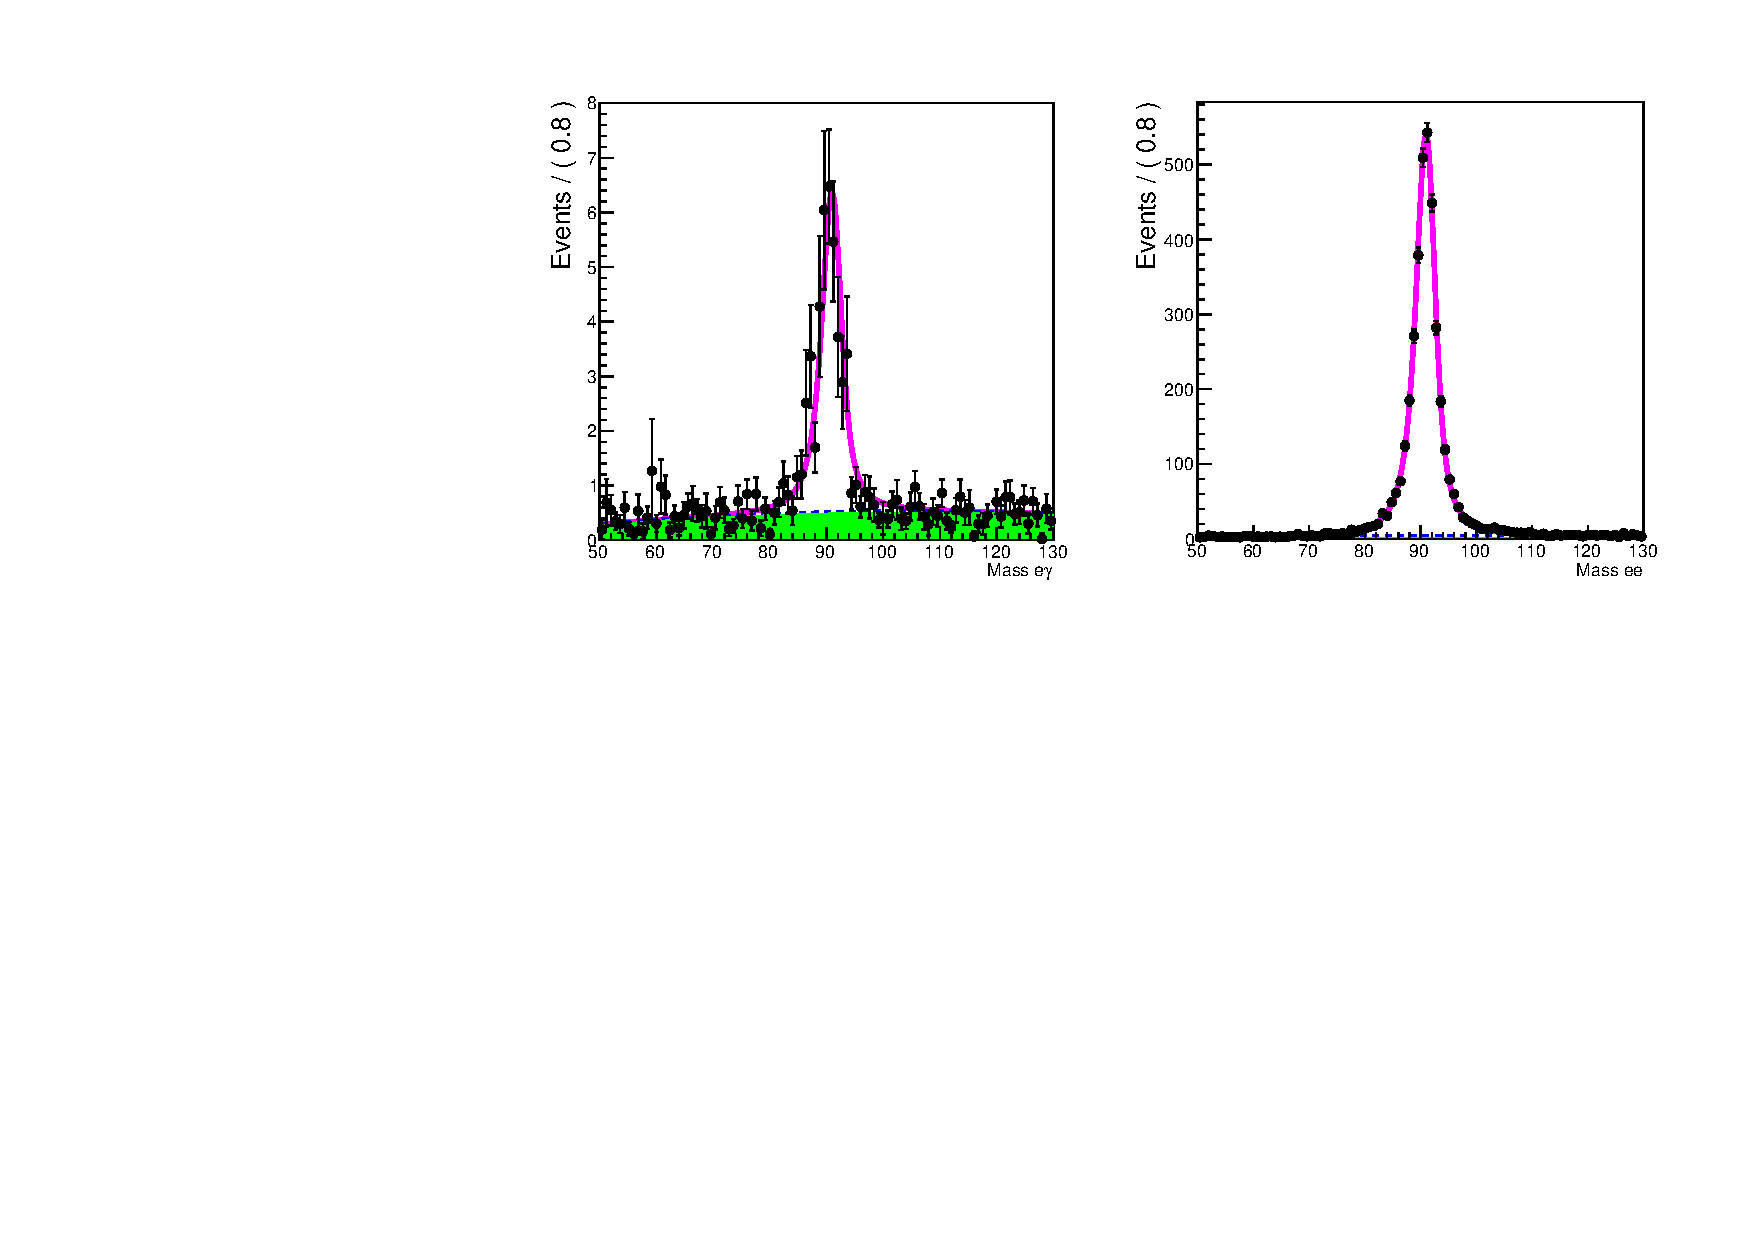
\includegraphics[width=0.48\linewidth]{../Figures/Chap3/fake_rate_tag_and_probe/tag_probe_MC_fit_qmult_0_1.pdf}
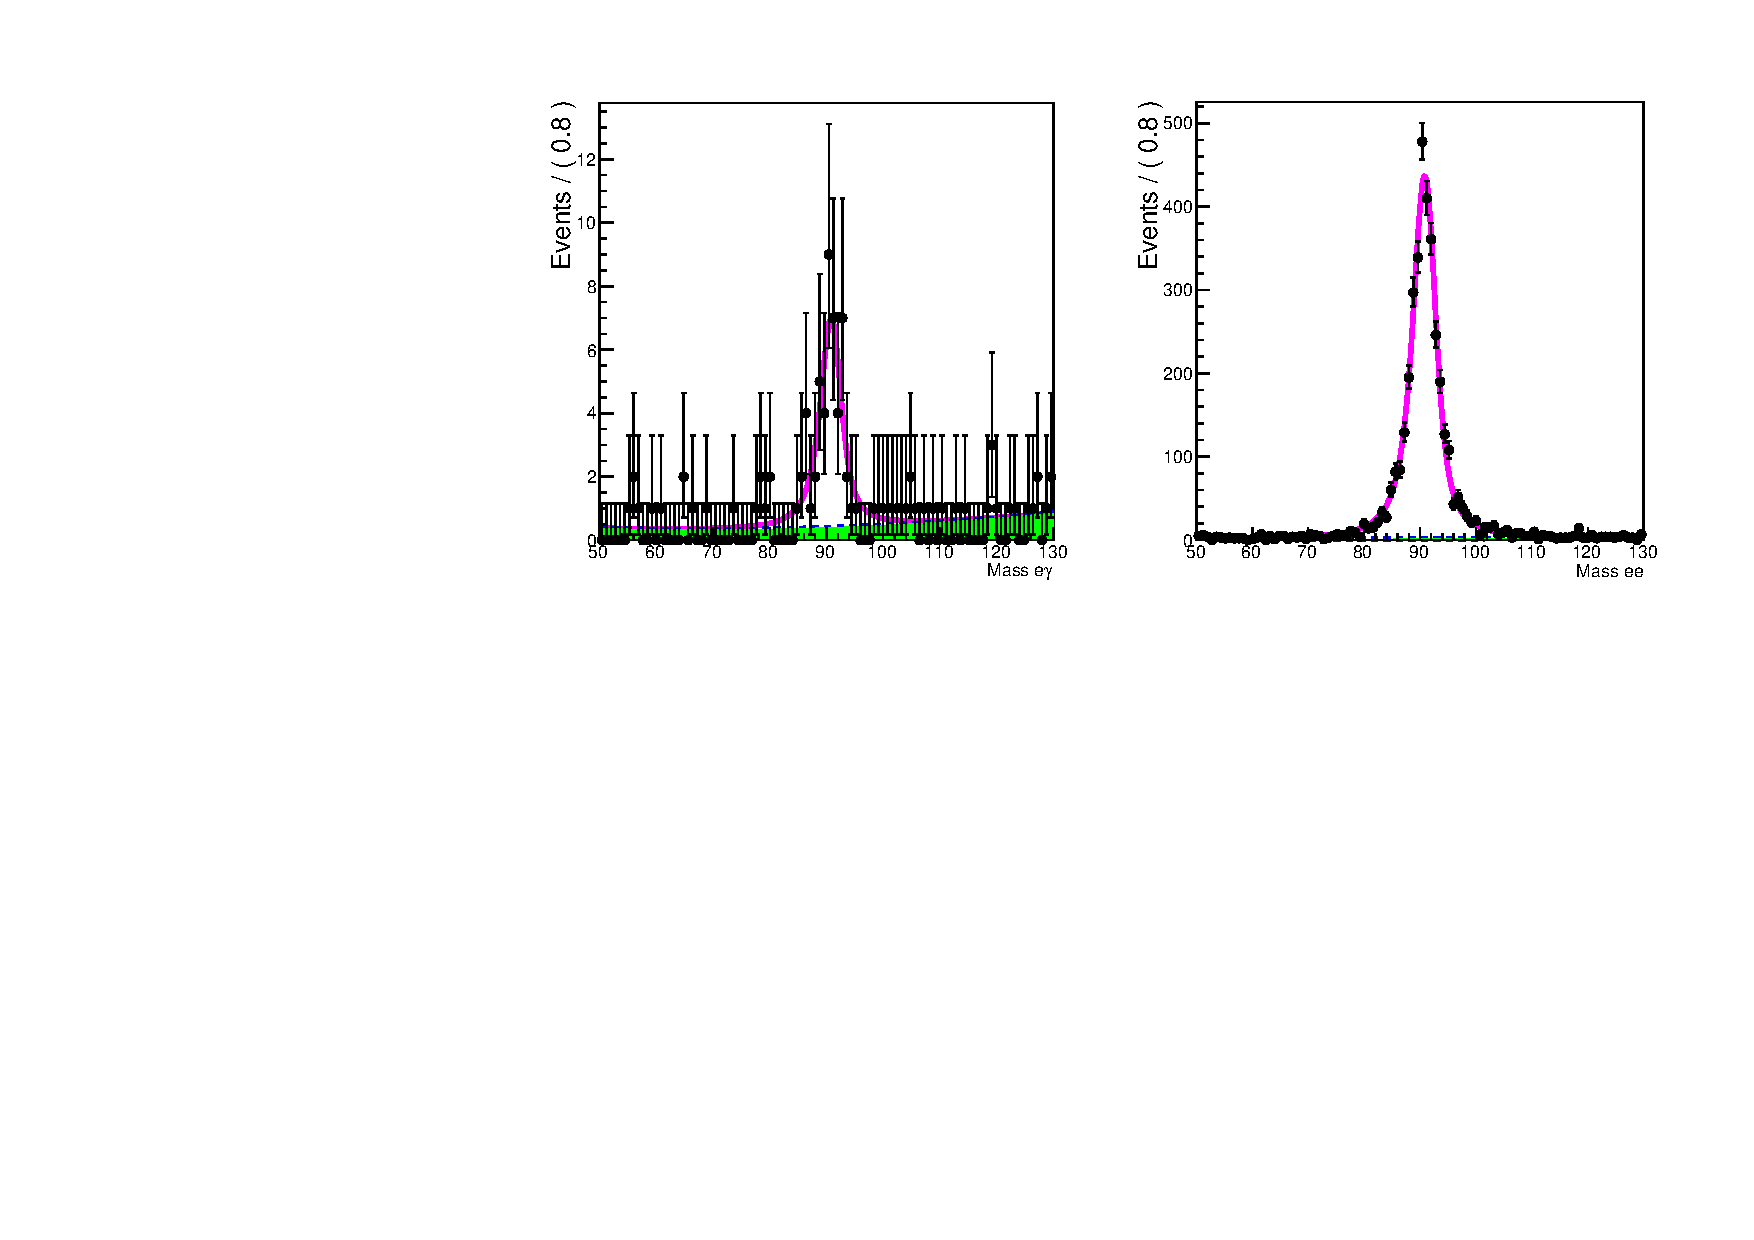
\includegraphics[width=0.48\linewidth]{../Figures/Chap3/fake_rate_tag_and_probe/tag_probe_fit_qmult_0_1.pdf}\\
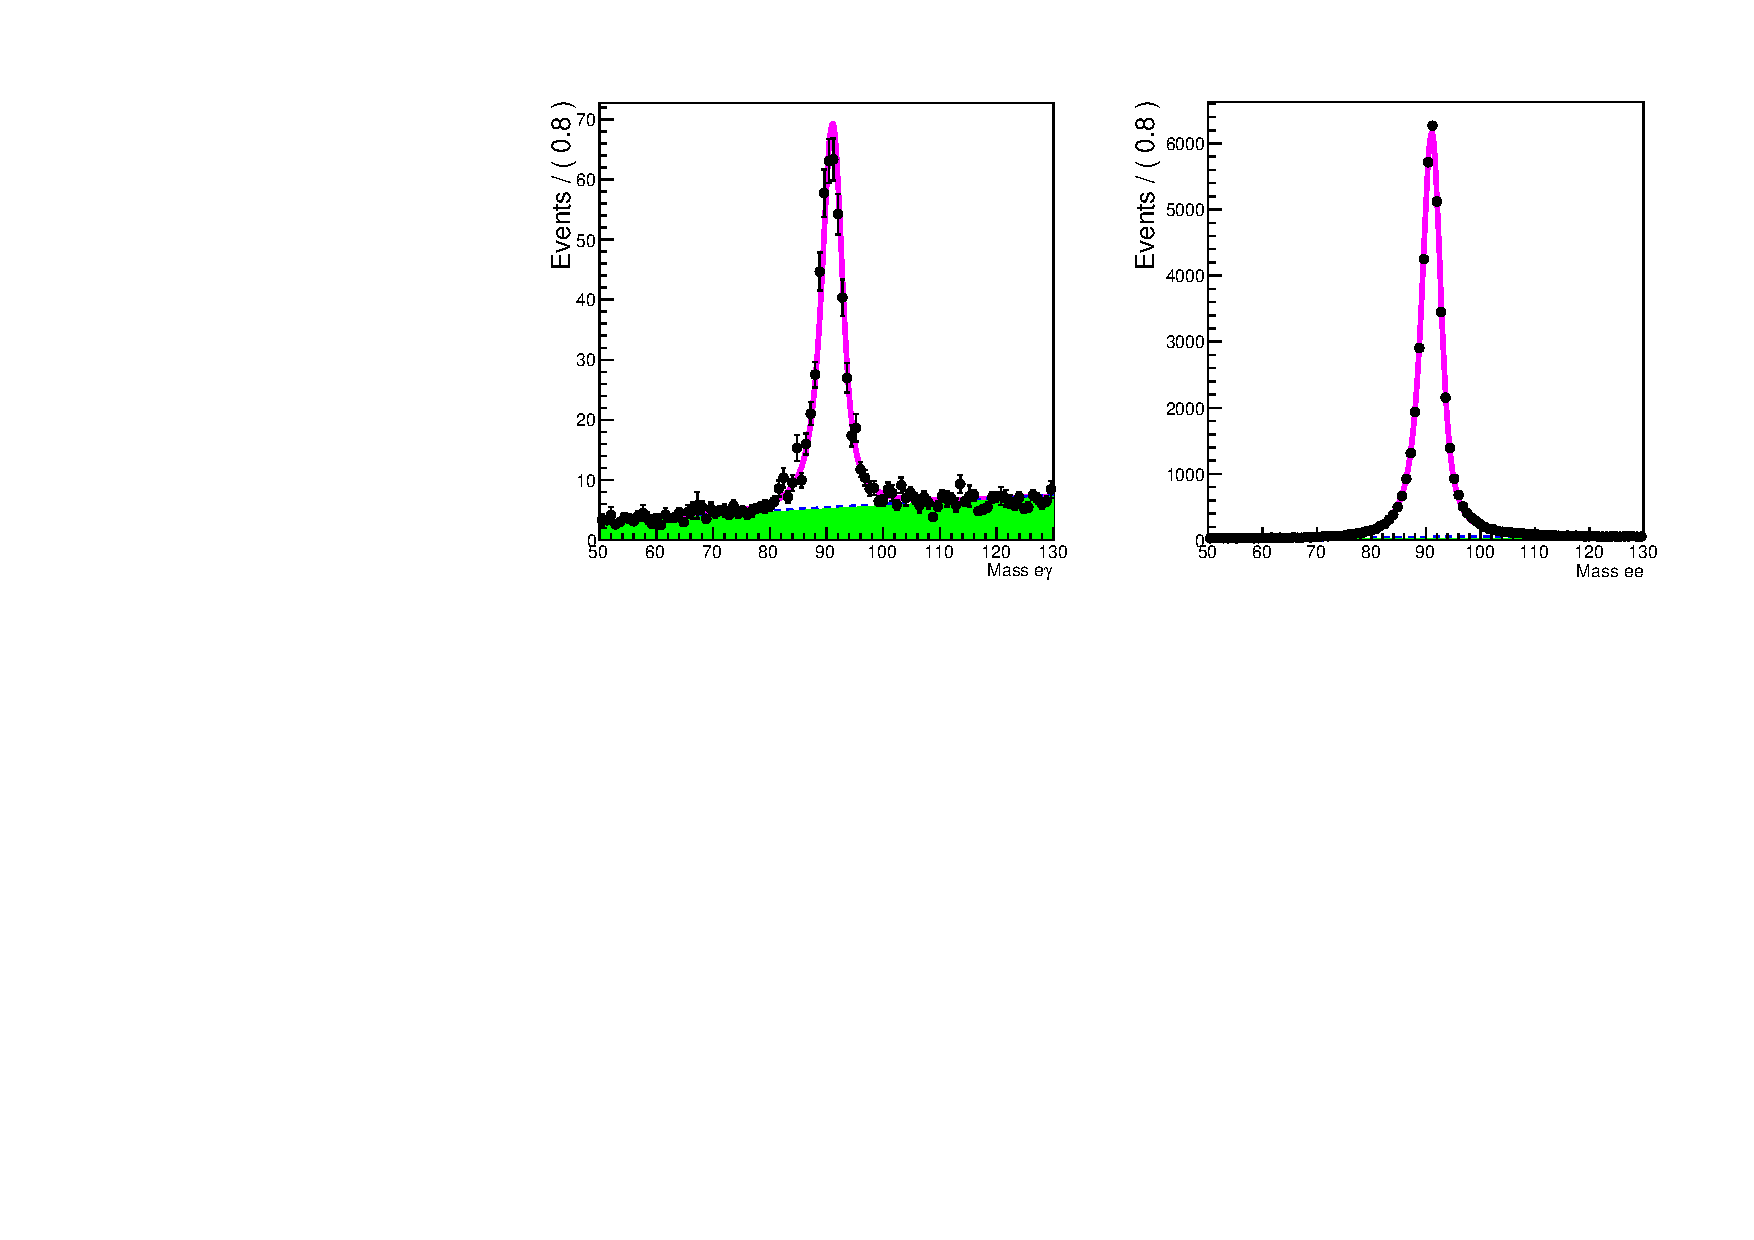
\includegraphics[width=0.48\linewidth]{../Figures/Chap3/fake_rate_tag_and_probe/tag_probe_MC_fit_qmult_2_100.pdf}
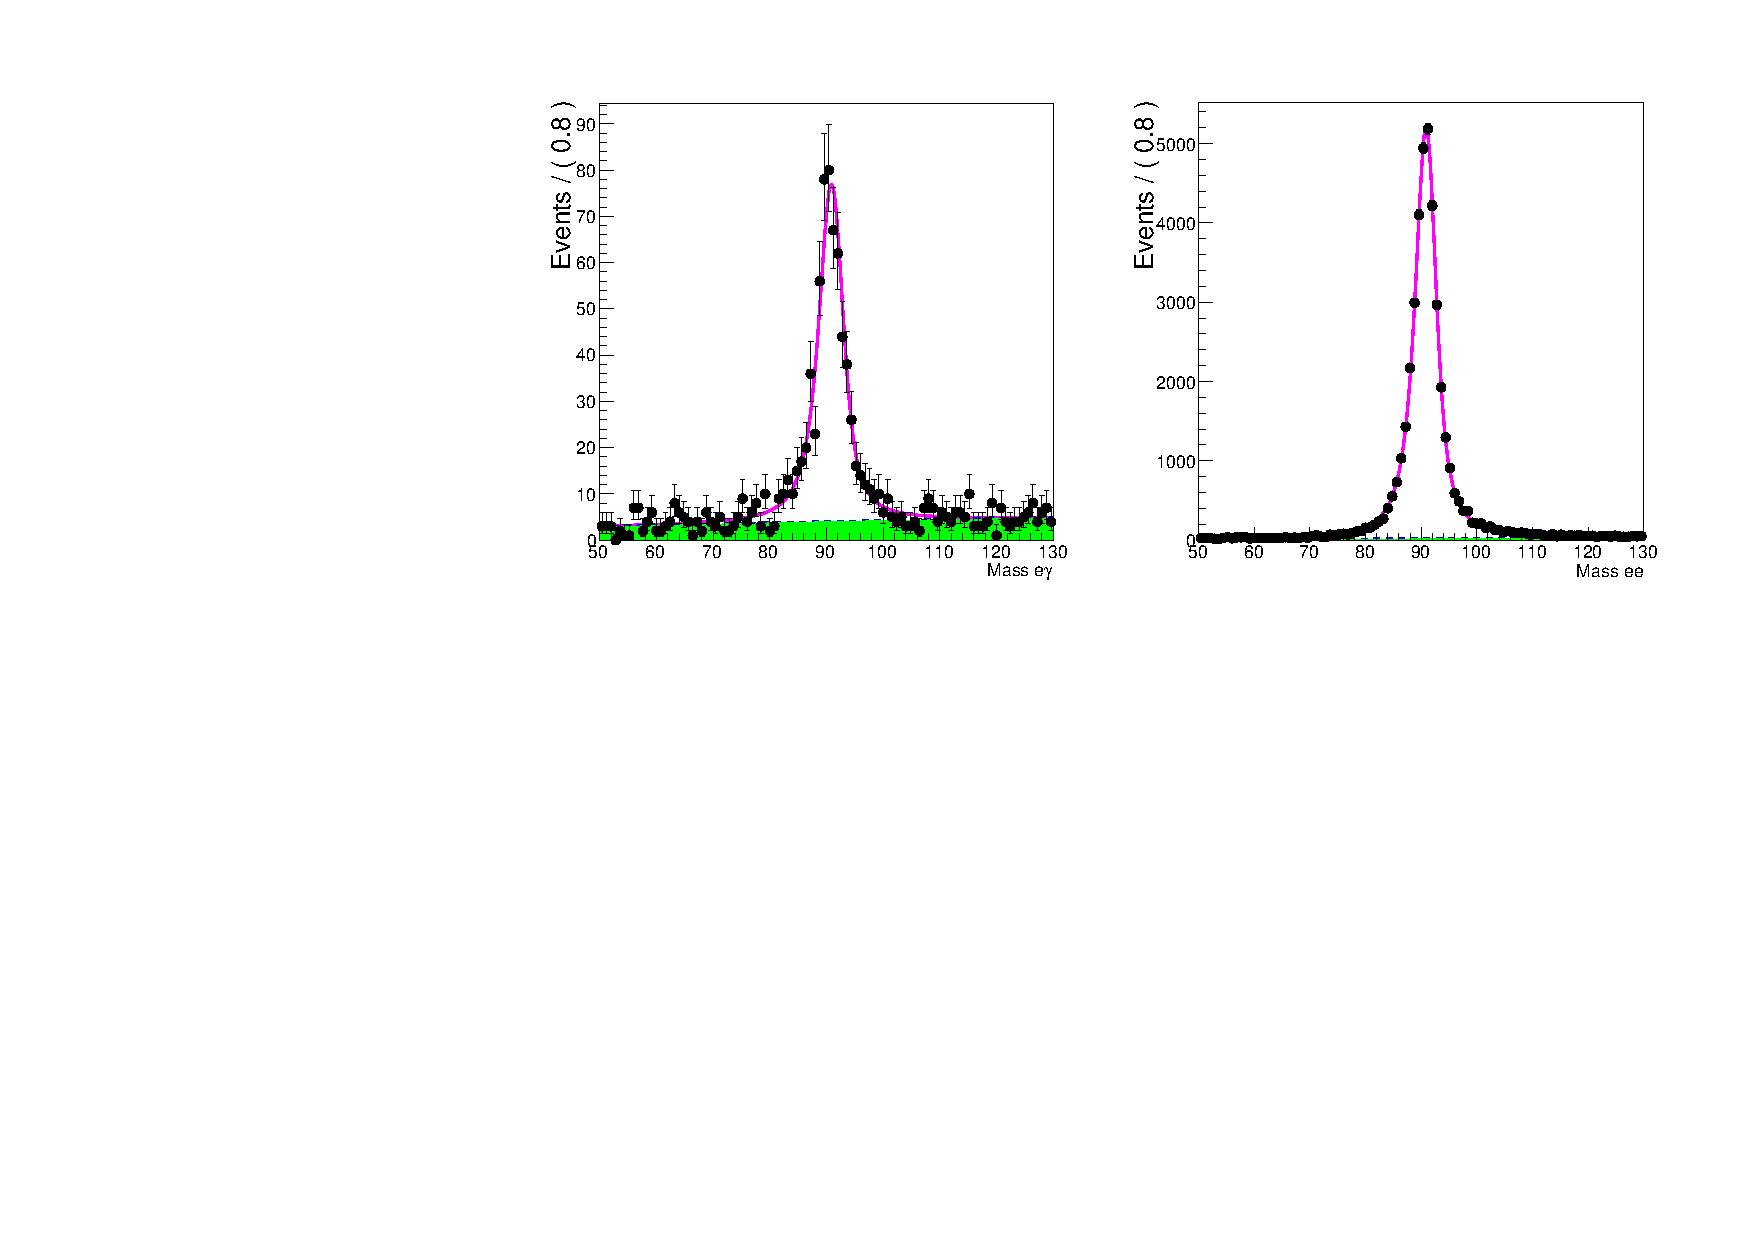
\includegraphics[width=0.48\linewidth]{../Figures/Chap3/fake_rate_tag_and_probe/tag_probe_fit_qmult_2_100.pdf}\\
\captionsetup{width=.9\linewidth}
\caption[Tag \& probe fits for data and MC]{Tag \& probe fits of the fake rate in 0-1 $Q_{mult}$ bins (top row) and $\geq2\ Q_{mult}$ bins (bottom row).
The first and second columns are the
the photon region and electron region fits in MC, respectively. The third and fourth columns are 
the photon region and electron region fits in data, respectively.}
\label{fig:tpFits}
\end{figure}

\subsubsection{Fake rate prediction}
Using the results described above, the prediction for the fake photon background is shown in 
Table~\ref{tab:fakeRatePredictions} (for high \dphi) and Table~\ref{tab:fakeRatePredictions_LDP} (for low \dphi).
\subsection{Invisible Z estimation}
\label{subsec:zinv}
The invisible Z background is estimated using a $Z(\ell\ell)$ plus $\gamma$ control region.
The method relies on the fact that for $\gamma Z(\nu\nu)$ events, the \ptmiss is
roughly equal to the transverse momentum of the Z boson.  There is also a small
contribution from limited resolution
of other objects in the event -- primarily jets; this effect of finite resolution
means that $p_{T,Z(\ell\ell)}$ cannot be used directly as a proxy for \ptmiss.   

The $Z(\ell\ell)$ plus $\gamma$ events are required to have one high-\pt photon and two oppositely 
charged, same flavor leptons (e, $\mu$) whose invariant mass is consistent with 
the Z mass, $80<m_{\ell\ell}<100~\gev$.  For the purposes of computing event level
kinematic variables, the effect of leptons is removed.  For \ST, \nj, \nb, and $\dphi$
jets which are matched, $\Delta R<0.3$, to the charged leptons are ignored.  For \ptmiss
the reconstructed transverse momentum of the Z candidate is added to the \ptmiss vector.
This cleaning procedure allow for finite jet resolution to smear the $p_{T,Z(\ell\ell)}$
and provide a consistent way of modeling the kinematics of neutrino decays.  The kinematic 
selections are then the same as the signal region, but using these ``cleaned'' variables.  

$Z(\ell\ell)$ plus $\gamma$ events have one primary difference with respect to $Z(\nu\nu)+\gamma$
events;  the former can result from the photon being radiated by charged leptons from the
Z boson decay.  This effect is small for our phase space, $p_{T,Z(\ell\ell)}$~\ptmiss$>100~\gev$ and 
$\ptg>100~\gev$.  However, these events will typically produce a photon which is
roughly colinear with one of the charged leptons in the event.  We require that the angle 
between any electron or muon and the photon be $\Delta R(e/\mu,\gamma)>0.2$. We also 
require invariant mass of di-lepton pair to be in the range $80-100\ \gev$ which further supresses 
the photon radiation from lepton.

The triggers for the $\gamma$-DY control region are the same as the signal region
triggers.

Because of the low statistics for Z($\ell\ell$)+$\gamma$ events, the \ptmiss shape will be taken directly from MC.  
The overall event yield will be measured by scaling the $Z(\nu\nu)+\gamma$ event yield
by a MC transfer factor, TF, ($N^{\text{MC}}_{\nu\nu+\gamma}/N_{ll+\gamma}^{\text{MC}}$) that will account for the relative branching ratio, $\mathcal{B}(\nu\nu)/\mathcal{B}(\ell\ell)$,
and reconstruction efficiencies of the charged leptons. The kinematics of the Z($\nu\nu$)+$\gamma$ and Z($\ell\ell$)+$\gamma$ are very identical
and they are shown in figure \ref{fig:ZGTF} for some of the variables. 
Because of the nonavailability of the Z($\ell\ell$)+$\gamma$ MC 
samples with $\ptg<130~\gev$, these transfer factors are derived from high $\ptg$ region.

The prediction is given by,
\begin{equation}
\label{eq:zgamma}
  \centering
  N_{\nu\nu+\gamma}^{data}(SR\ Bin) = N_{ll+\gamma}^{data}\cdot \beta_{ll+\gamma}\cdot  \bigg( \frac{N^{\text{MC}}_{\nu\nu+\gamma}}{N_{ll+\gamma}^{\text{MC}}} \bigg)^{p^T_\gamma > 190}\cdot \frac{N^{\text{MC}}_{\nu\nu+\gamma}(SR\ Bin)}{N^{\text{MC}}_{\nu\nu+\gamma}}
\end{equation}
where $\beta_{\ell\ell+\gamma}$ represents the purity of the Z($\ell\ell$)+$\gamma$ control
region and the last term $N_{\nu\nu+\gamma}^{\text{MC}}(SR\ Bin)/N^{\text{MC}}_{\nu\nu+\gamma}$ 
represents a MC template that determines the 
\ptmiss,\nj shape of the prediction; the template is computed independently for each 
of the signal regions. $N_{\ell\ell+\gamma}^{data}$ represents the
observed number of events in data while $N_{\ell\ell+\gamma}^{\text{MC}}$ represents 
the expected number of from MC; both are computed inclusively in search bins. 
As mentioned before, we derive TF in $p_T^{\gamma} > 190\ \gev$ region. There are two reasons why the same TF is applicable even at low photon \ptg regions:\\

\begin{itemize}
\item The number of events that lie in the region $100 < p_T^{\gamma} < 190\gev$ is a small fraction of the total events (about 15\%).
\item TF is not dependent on photon $p_T$ (top left plot in Figure \ref{fig:ZGTF}).
\end{itemize}

\begin{figure}[h!]
\centering
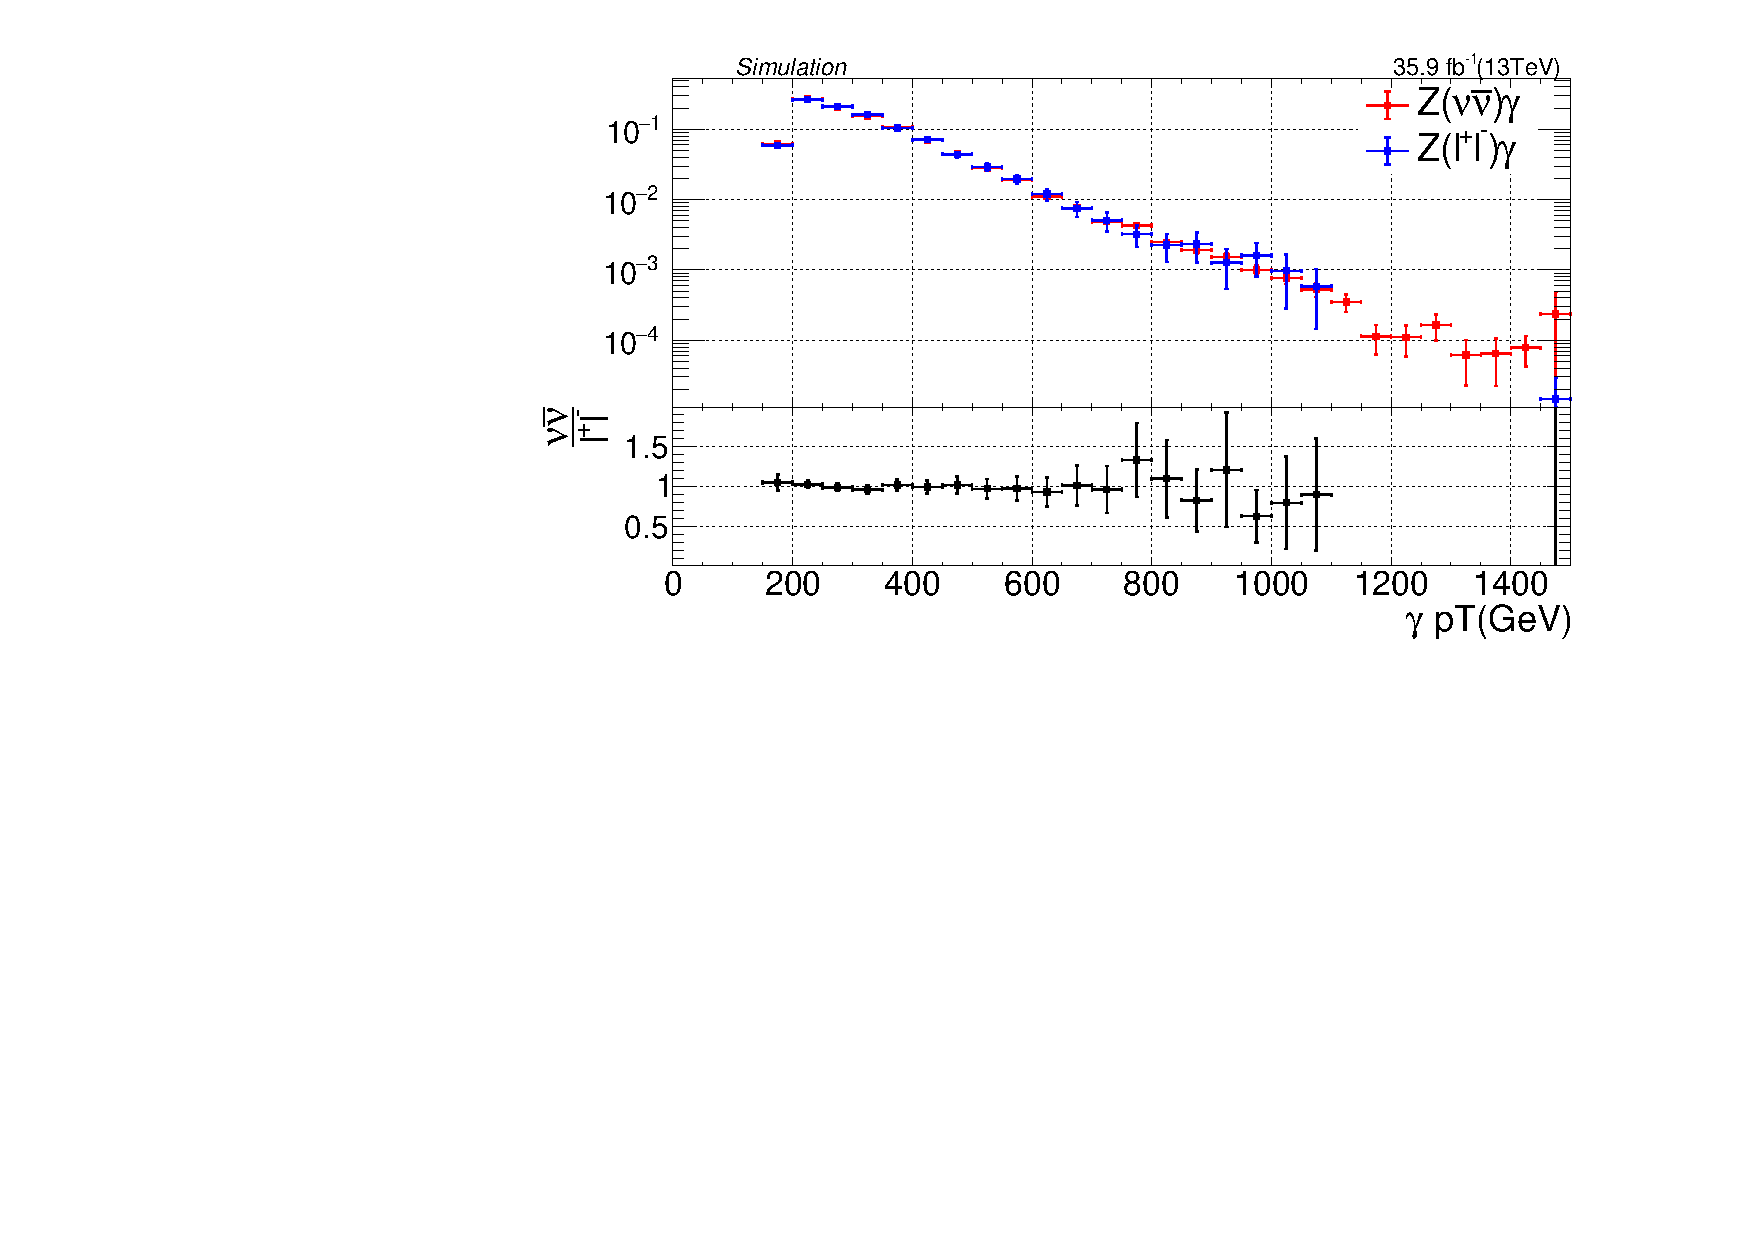
\includegraphics[width=0.48\linewidth]{../Figures/Chap3/zgamma/BestPhotonPtNuNu_LL_LO.pdf}
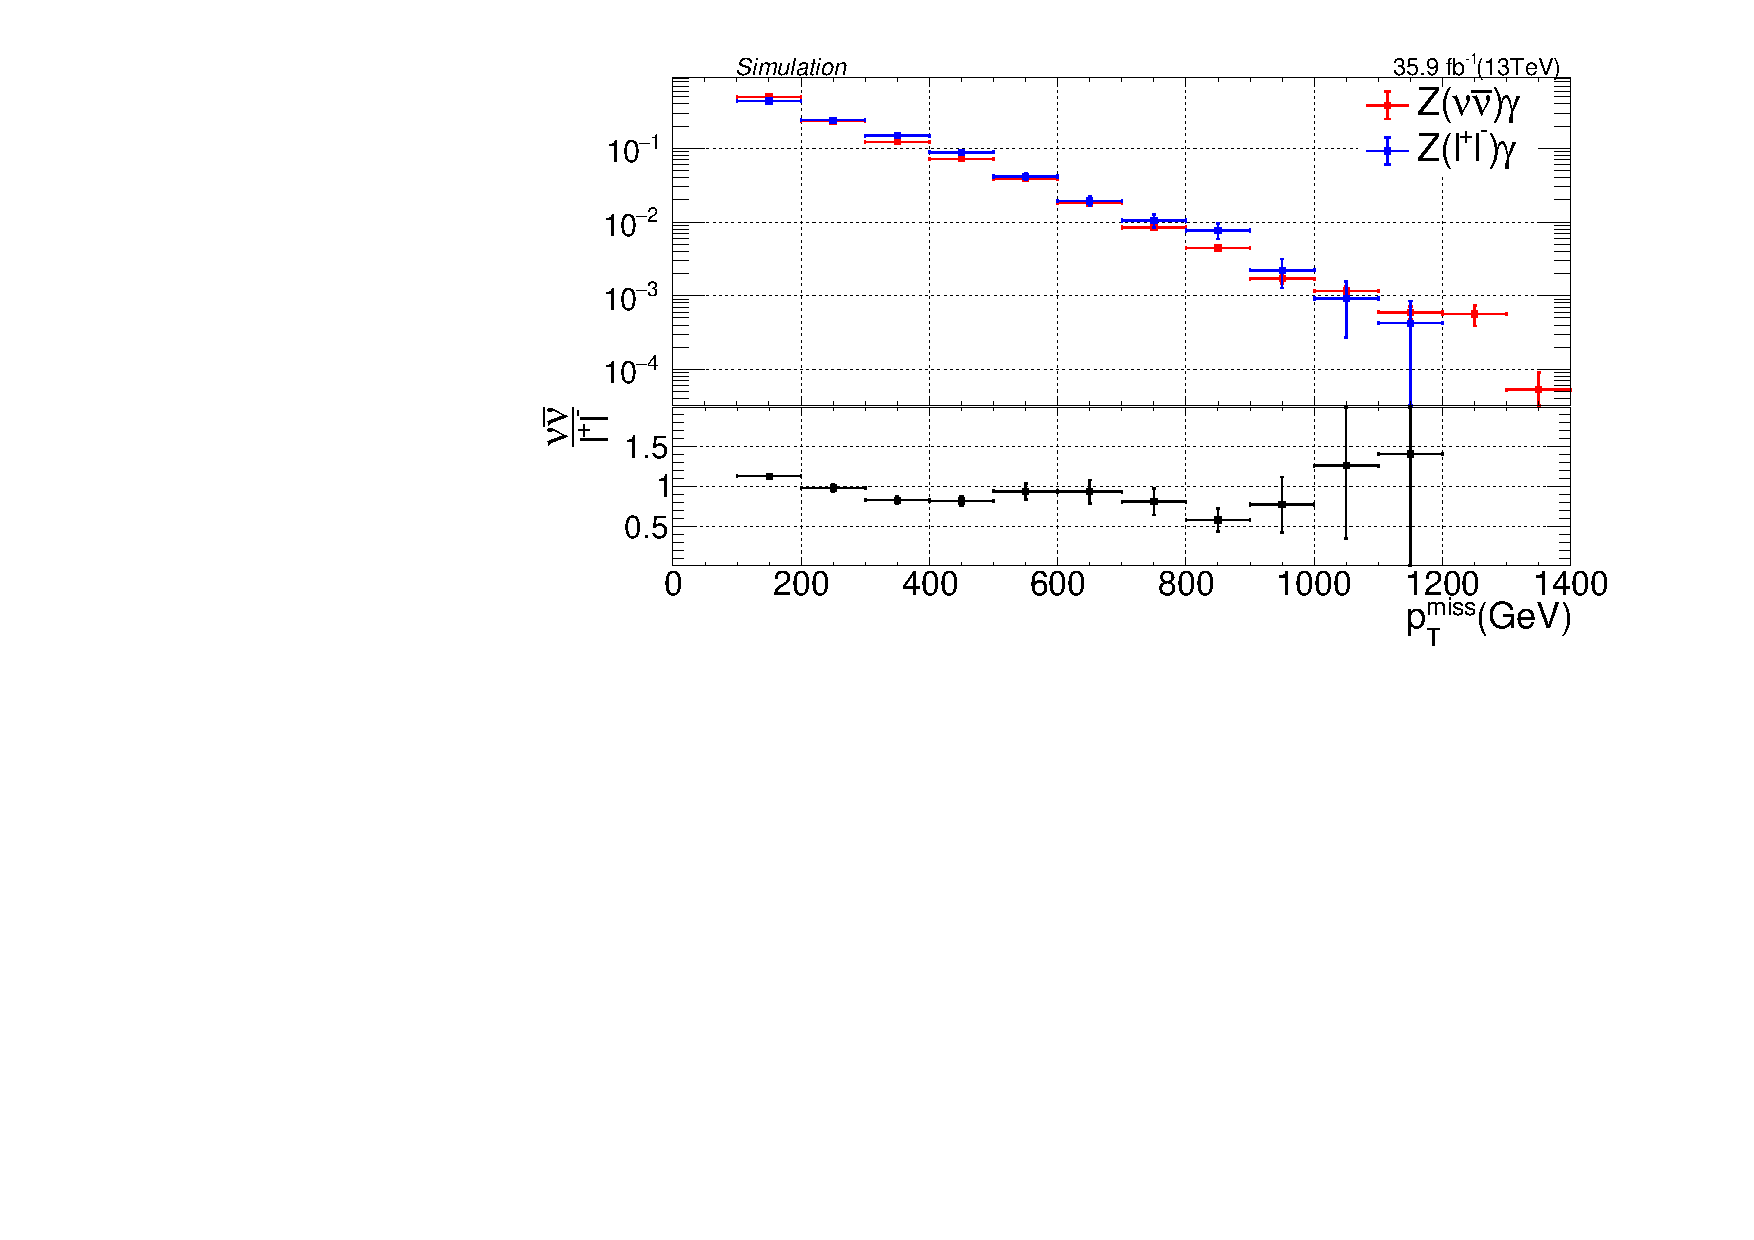
\includegraphics[width=0.48\linewidth]{../Figures/Chap3/zgamma/METNuNu_LL_LO.pdf}\\
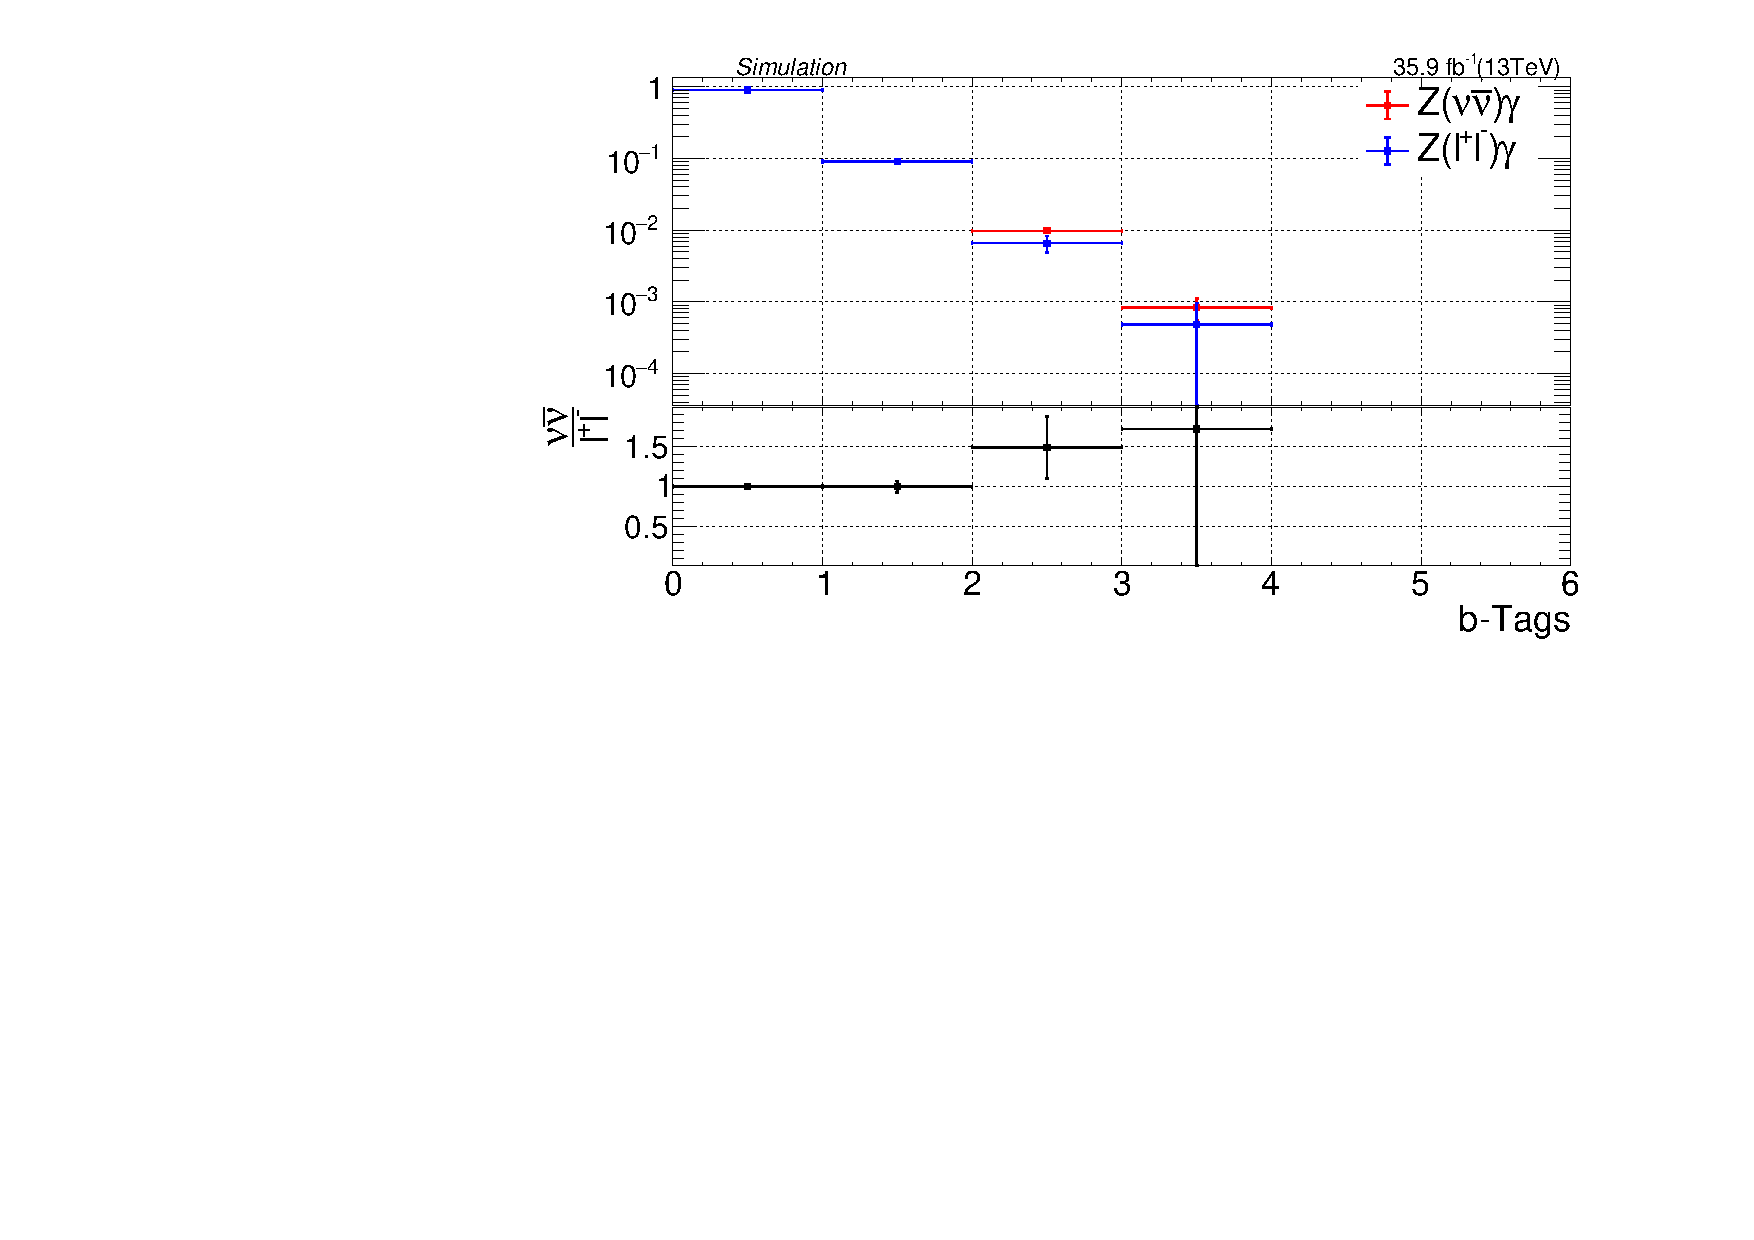
\includegraphics[width=0.48\linewidth]{../Figures/Chap3/zgamma/nBTagsNuNu_LL_LO.pdf}
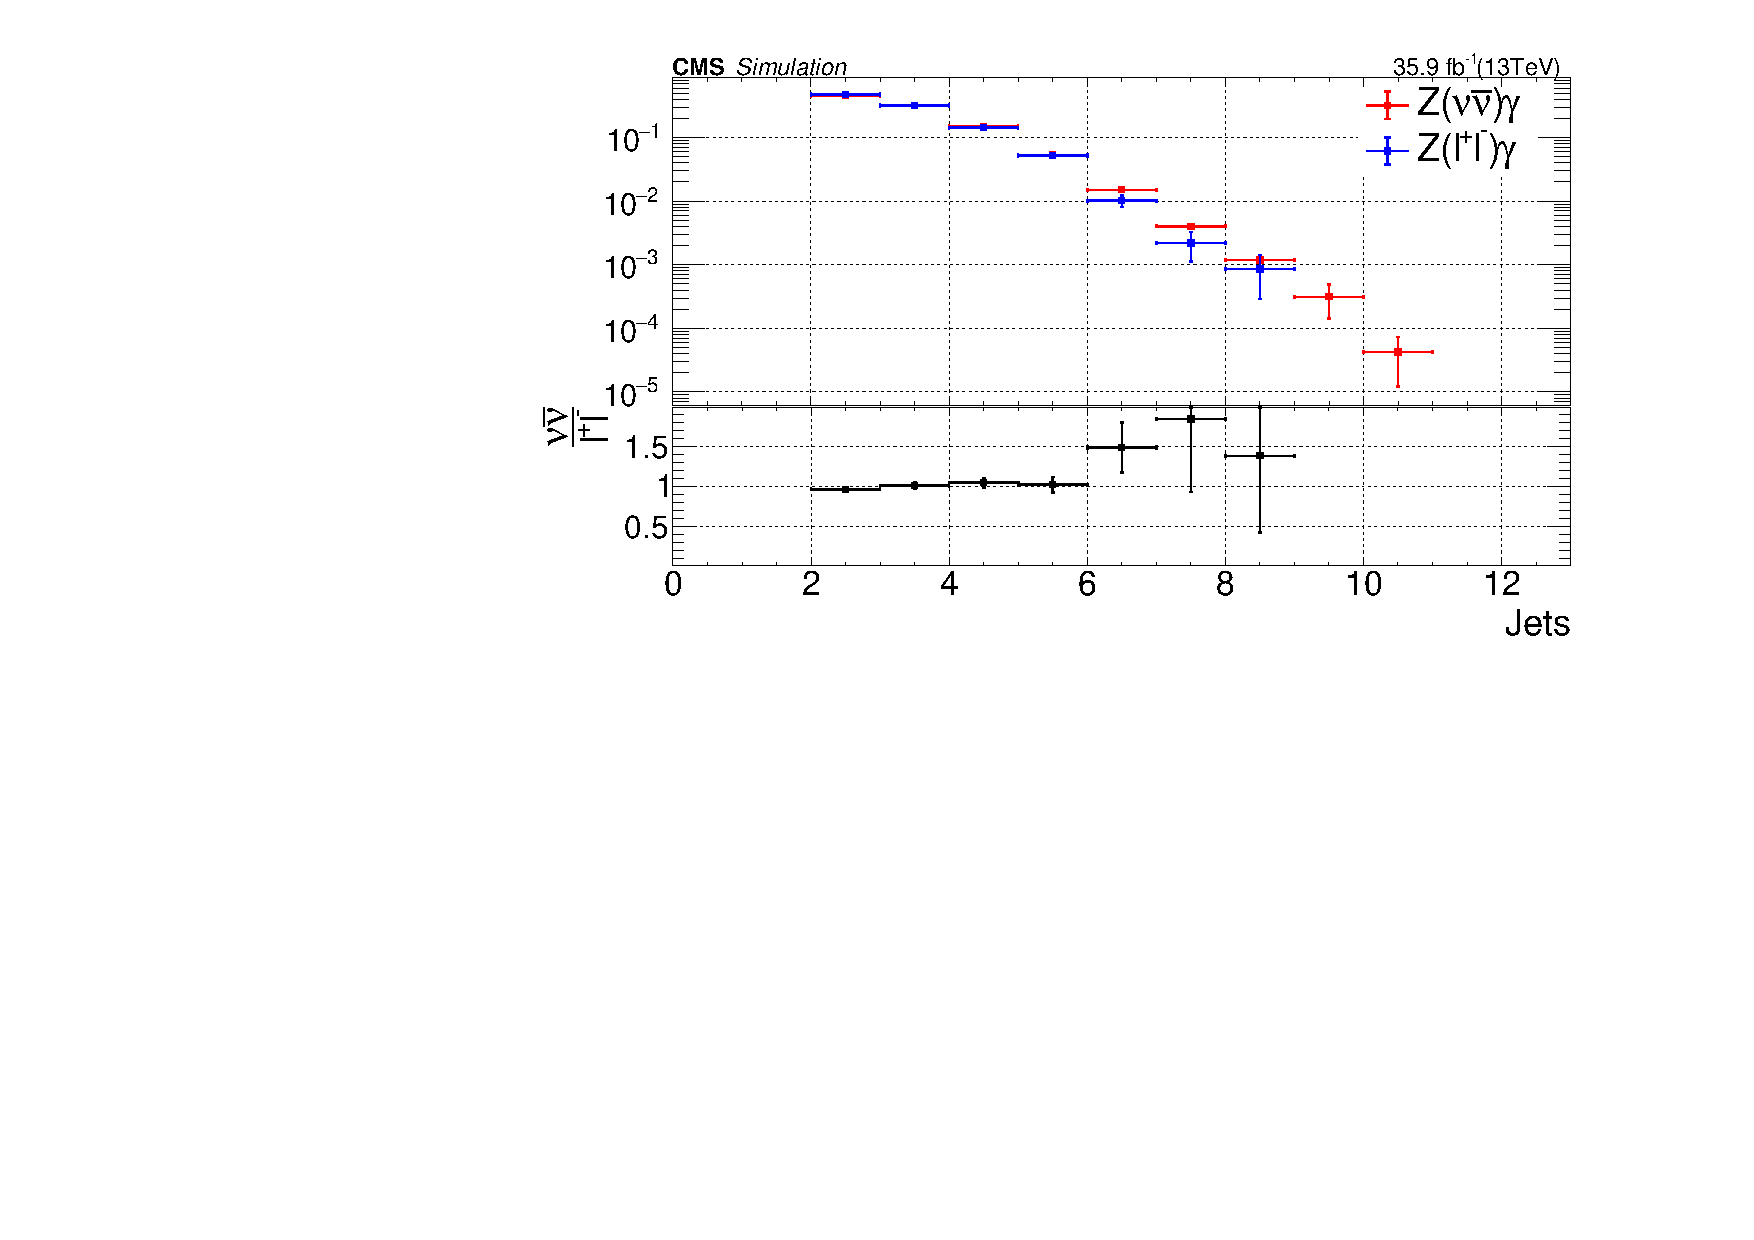
\includegraphics[width=0.48\linewidth]{../Figures/Chap3/zgamma/nHadJetsNuNu_LL_LO.pdf}
\caption[Comparing $Z(ll)\gamma$ with $Z(\nu\nu)\gamma$]{Comparison of $Z(ll)\gamma$ with $Z(\nu\nu)\gamma$ as function of \ptg (top left), \ptmiss (top right), \nb (bottom left) and \nj (bottom right) for $\ptg>190\ \gev$}
\label{fig:ZGTF}
\end{figure}

The purity of the Z($\ell\ell$)+$\gamma$ control region is determined from a fit 
to the invariant mass, $m_{\ell\ell}$, distribution.  This isolates contamination 
from $\gamma t\bar{t}$ events, which are expected to have a roughly flat distribution.
The purity is checked in three different ways, using MC to predict the number of 
$t\bar{t}\gamma$ events, using a fit to the $m_{\ell\ell}$ distribution, and
using the opposite-sign, different-flavor control sample ($e\mu\gamma$).  All three
prediction give consistent results when calculated within the baseline phase-space, 
which are reported in Table~\ref{tab:zGammaPurity}. 
%Figure~\ref{fig:DYgammaPurity} 
%shows the observed $m_{\ell\ell}$ distribution plus the fitted mass spectrum. 
The uncertainties associated with our prediction of the 
$Z(\ell\ell)\gamma$ purity is also propagated to the final 
$Z\gamma$ prediction. 

%\begin{figure}
%\centering
%\includegraphics[width=0.48\linewidth]{../Figures/Chap3/zgamma/ZgammaPurityFit.png}
%\caption{Distribution of $m_{\ell\ell}$ for data and MC.  All events shown are required
%to pass the DY-$\gamma$ selections.}
%\label{fig:DYgammaPurity}
%\end{figure}

\begin{table}[h!]
\centering
\caption{Purity in the $Z\gamma$ control region.}
\label{tab:zGammaPurity}
\begin{tabular}{c|c|c|c}
\hline
         & \multicolumn{3}{c}{Method} \\\cline{2-4}
\nb      & MC              & $m_{\ell\ell}$ fits & $e\mu$ CR \\\hline\hline
%$=0$     & 0.995 $\pm$ 0.005  & -    & 0.968 $\pm$ 0.032  & 0.99 $\pm$ 0.01 \\\hline
%$\geq 1$ & 0.844 $\pm$ 0.065  & -    & 1.0   $\pm$ 0.0    & 0.84 $\pm$ 0.16 \\ \hline  
$\geq 0$ & 0.978 $\pm$ 0.009  & 0.97 & 0.97 $\pm$ 0.03   \\\hline
\end{tabular}
\end{table}

Because of the very low statistics in low \dphi region in data, we make use of scale factors that are derived using high \dphi events to predict events in the low \dphi region. Scale factor is given by equation \ref{eqn:ZGSF} and it is found to be $1.11\pm0.21$.
\begin{equation}
\label{eqn:ZGSF}
SF = \bigg(\frac{N_{ll+\gamma}^{data}\cdot \beta_{ll+\gamma}}{N^{\text{MC}}_{\nu\nu+\gamma}}\bigg)^{p^T_\gamma > 190,high\ \dphi}
\end{equation}
Prediction in low \dphi region is,
\begin{equation}
N_{\nu\nu+\gamma}^{data}(SR\ Bin) = SF\cdot N^{\text{MC}}_{\nu\nu+\gamma}(SR\ Bin)
\end{equation}
%For 0 b-tag SF is $1.10\pm0.22$ and for $\geq$ 1 b-tag region SF is $1.38\pm0.72$.

To account for systematic uncertainties associated with the MC
modeling of the \ptmiss shape, we apply the full electro-weak corrections obtained from 
theory calculations \cite{Denner:2015fca} as a function of \ptmiss. These uncertainties are listed in table \ref{tab:EWcorr}.
they can be as high as 40\% in highest \ptmiss bin. These uncertainties are treated as
correlated across \ptmiss bins for the limit setting procedure. Uncertainties from b-tag SF are also considered and they are 2\% in 0b-tag bins and 6\% in $\geq1$b-tag bins. The b-tag SF uncertainty is treated as anti-correlated in 0 and $\geq1$ b-tag bins. Final predictions for Z$(\nu\nu)+\gamma$ are listed in Table \ref{tab:znnPredictions} for high \dphi and in Table \ref{tab:znnLDPPredictions} for low \dphi regions.

\begin{table}[h!]
\centering
\caption{Electroweak corrections as a function of \ptmiss.}
\label{tab:EWcorr}
\begin{tabular}{|c|c|}
\hline  \ptmiss~(GeV) & \% EW Correction  \\ 
\hline  100-200 &  8\\ 
\hline  200-270 &  18\\ 
\hline  270-350 &  20\\ 
\hline  350-450 &  25\\ 
\hline  450-750 &  35\\ 
\hline  $\geq$ 750&  40\\ 
\hline 
\end{tabular}
\end{table} 

\subsection{\gjets and QCD multijet estimation}   

Along with the presence of a well identified high \pt photon in the event, the \gjets production contributes to the background in search regions if one of the jets in an event is mis-measured resulting in fake \ptmiss or it contains a jet originating from b-quarks with a semileptonic decay of B mesons. Fluctuations in hadronization of jets can also result in an energetic $\pi^0$ misidentified as a photon which along with fake \ptmiss originating from other jets in the event can result in a QCD multijet production contribution to the search regions. Fake \ptmiss arising from mis-measurements of jets or semileptonic b-jets is usually aligned with the jet itself. Hence, a most of this background is rejected by angular cuts summarized in section \ref{sec:event-selection} i.e. \dphi(\ptvecmiss, \ptvecjet) $>$ 0.3 for first two leading jets. The main contribution to background is due to the \gjets processes and QCD multijet contribution is very small. In the method described in this section, the total background due to fake \ptmiss is estimated without further separating the QCD multijet and \gjets processes. 
The control sample to estimate the \gjets and QCD multijet background is derived inverting the \dphi(\ptmiss, jet1) and \dphi(\ptmiss, jet2) criteria (min($\dphi_{1},\dphi_{2}$) $<0.3$) while keeping all the search selections intact except that 100 $<$ \ptmiss $<$ 200~\gev sideband is also used.  Since fake \ptmiss and mis-measured jets are mostly aligned in transverse direction, the inverted \dphi region provides a high statistics region rich in multijet background. Figure \ref{fig:supp_Sim_mindPhi1dPhi2_T5bbbbZG} shows the min($\dphi_{1},\dphi_{2}$) distribution in MC with \ptmiss $>200$ \gev. 
\begin{figure}[h!]
\centering
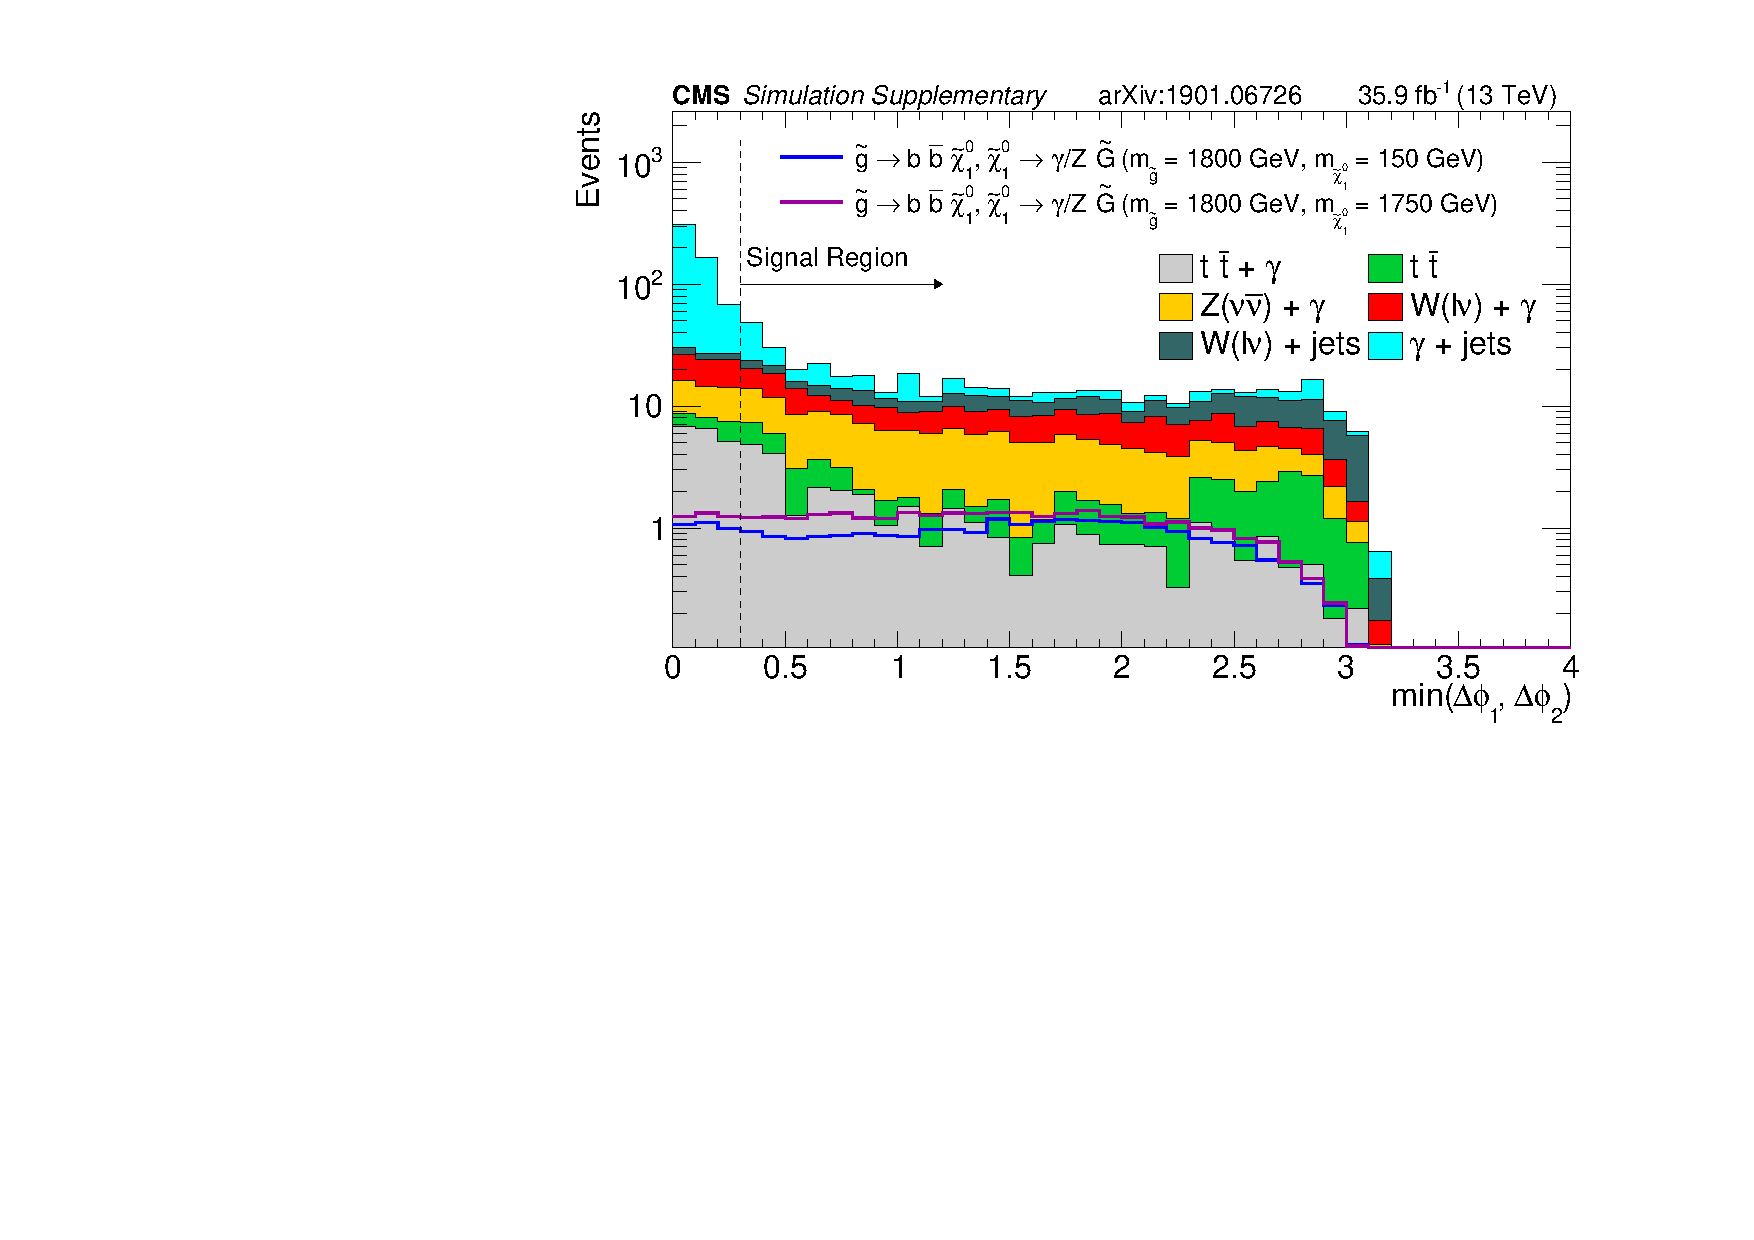
\includegraphics[width=0.8\linewidth]{../Figures/Chap3/anaPublic/supp_Sim_mindPhi1dPhi2_T5bbbbZG}
\captionsetup{width=.9\linewidth}
\caption[Min($\dphi_{1},\dphi_{2}$) in MC]{Distribution of min($\dphi_{1},\dphi_{2}$) in MC after applying all signal region selections except angular cuts. The region min($\dphi_{1},\dphi_{2}$) below 0.3 serves as a \gjets enriched sample and min($\dphi_{1},\dphi_{2}$) $>0.3$ is the signal region. In this plot, $\ptmiss > 200$ \gev selection is applied. The histograms shown as lines represent two signal models which indicate that there is negligible signal contamination.}
\label{fig:supp_Sim_mindPhi1dPhi2_T5bbbbZG}
\end{figure}

The method briefly summarized as follows: 
\begin{itemize}
 \item Using the low \ptmiss sideband, ratio R(\nj, \nb) = high-\dphi/low-\dphi is determined. This ratio is determined from data sideband. Contribution from electroweak background (lost lepton + \tauh, e faking photon and invisible Z) is subtracted from event yields before measuring the ratio. The R(\nj, \nb) means that the ratio is binned in the bins of jet multiplity and b-jet multiplicity.
 \item The number of events obtained in low-\dphi region in \ptmiss$>$200~\gev region, after subtracting the electroweak backgrounds, is multiplied with the ratio to obtained number of events in the search regions. 
 \item Since \dphi and \ptmiss are not completely independent, the method is corrected for dependence on \ptmiss using the MC, using an additional correction factor, $\kappa(\nj, \nb)$, where the quantities in bracket shows the binning variables. So in this sense, it is a ABCD method modified to correct for \dphi and \ptmiss dependencies using the $\kappa$ factor.
 \item The factor $\kappa$ is validated in data using zero photon events using jet with highest neutral electromagnetic fraction as a proxy to photon.
\end{itemize}

The boundaries for high-\dphi and low-\dphi, and high \ptmiss and low \ptmiss used as ABCD regions are shown in Figure~\ref{fig:abcd} (left). 
%Distribution of minimum of \dphi(\ptmiss, jet1) and \dphi(\ptmiss, jet2) versus \ptmiss in A, B, C, and D regions for \gjets and QCD multijet MC events which satisfy all other criteria for search region selection is shown in Figure~\ref{fig:abcd} (right).

\begin{figure}[h]
\centering
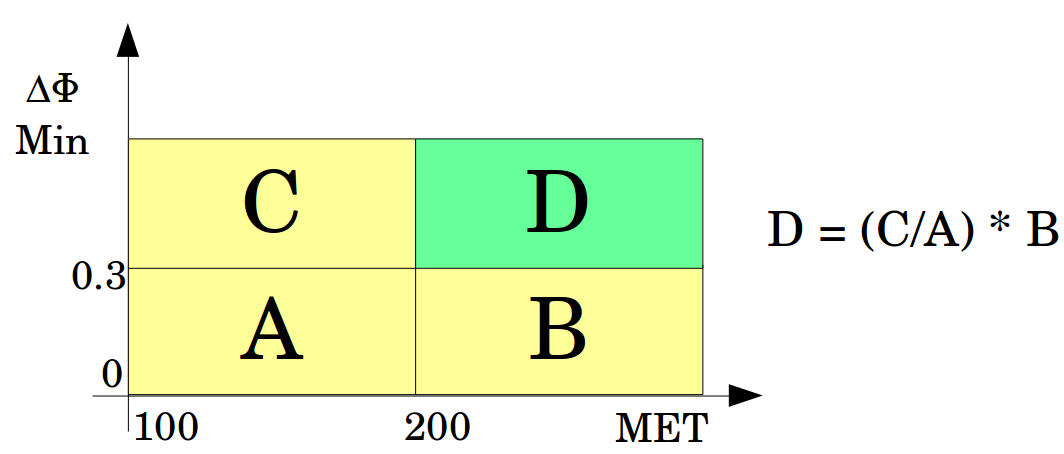
\includegraphics[width=0.48\linewidth]{../Figures/Chap3/SUSY_Photon_MET_JbJ_18Aug17/FakeMET/ABCD.png}
\caption[ABCD regions]{Definitions of various regions used in ABCD methods. Region D is signal region where background is to be estimated or validation region for zero photon sample.}
\label{fig:abcd}
\end{figure}

The ratio of high-\dphi to low-\dphi has a strong dependence as a function of \ptmiss. This dependence is accounted for by an additional correction factor using ratio, R, in low and high \ptmiss regions in MC. That is a factor $\kappa$ defined as \\
$\kappa$(\nj, \nb) = R(\nj, \nb) (high \ptmiss)/R(\nj, \nb)(low \ptmiss). \\
Please note that the ratio R and double ratio, $\kappa$ are binned in the bins of \nj and \nb. 

Using these values of R and $\kappa$, the performance of the method is validated using MC simulation. If the numbers R and $\kappa$ were derived using exact search region definitions, the closure would be one. Hence this validation mainly tests performance parameterization of these factors. The results of this closure tests are shown in Figure \ref{fig:qcdclosure} as a function of search bins used for this analysis. The number of \gjets and QCD multijet background events estimated using the methods (blue) closely reproduces those expected in search regions (cyan). The first bin in each \nj-\nb block corresponds to 100 $<$ \ptmiss $<$ 200~\gev control regions, where expected and predicted backgrounds exactly match by definition.

\begin{figure}[h!]
\centering
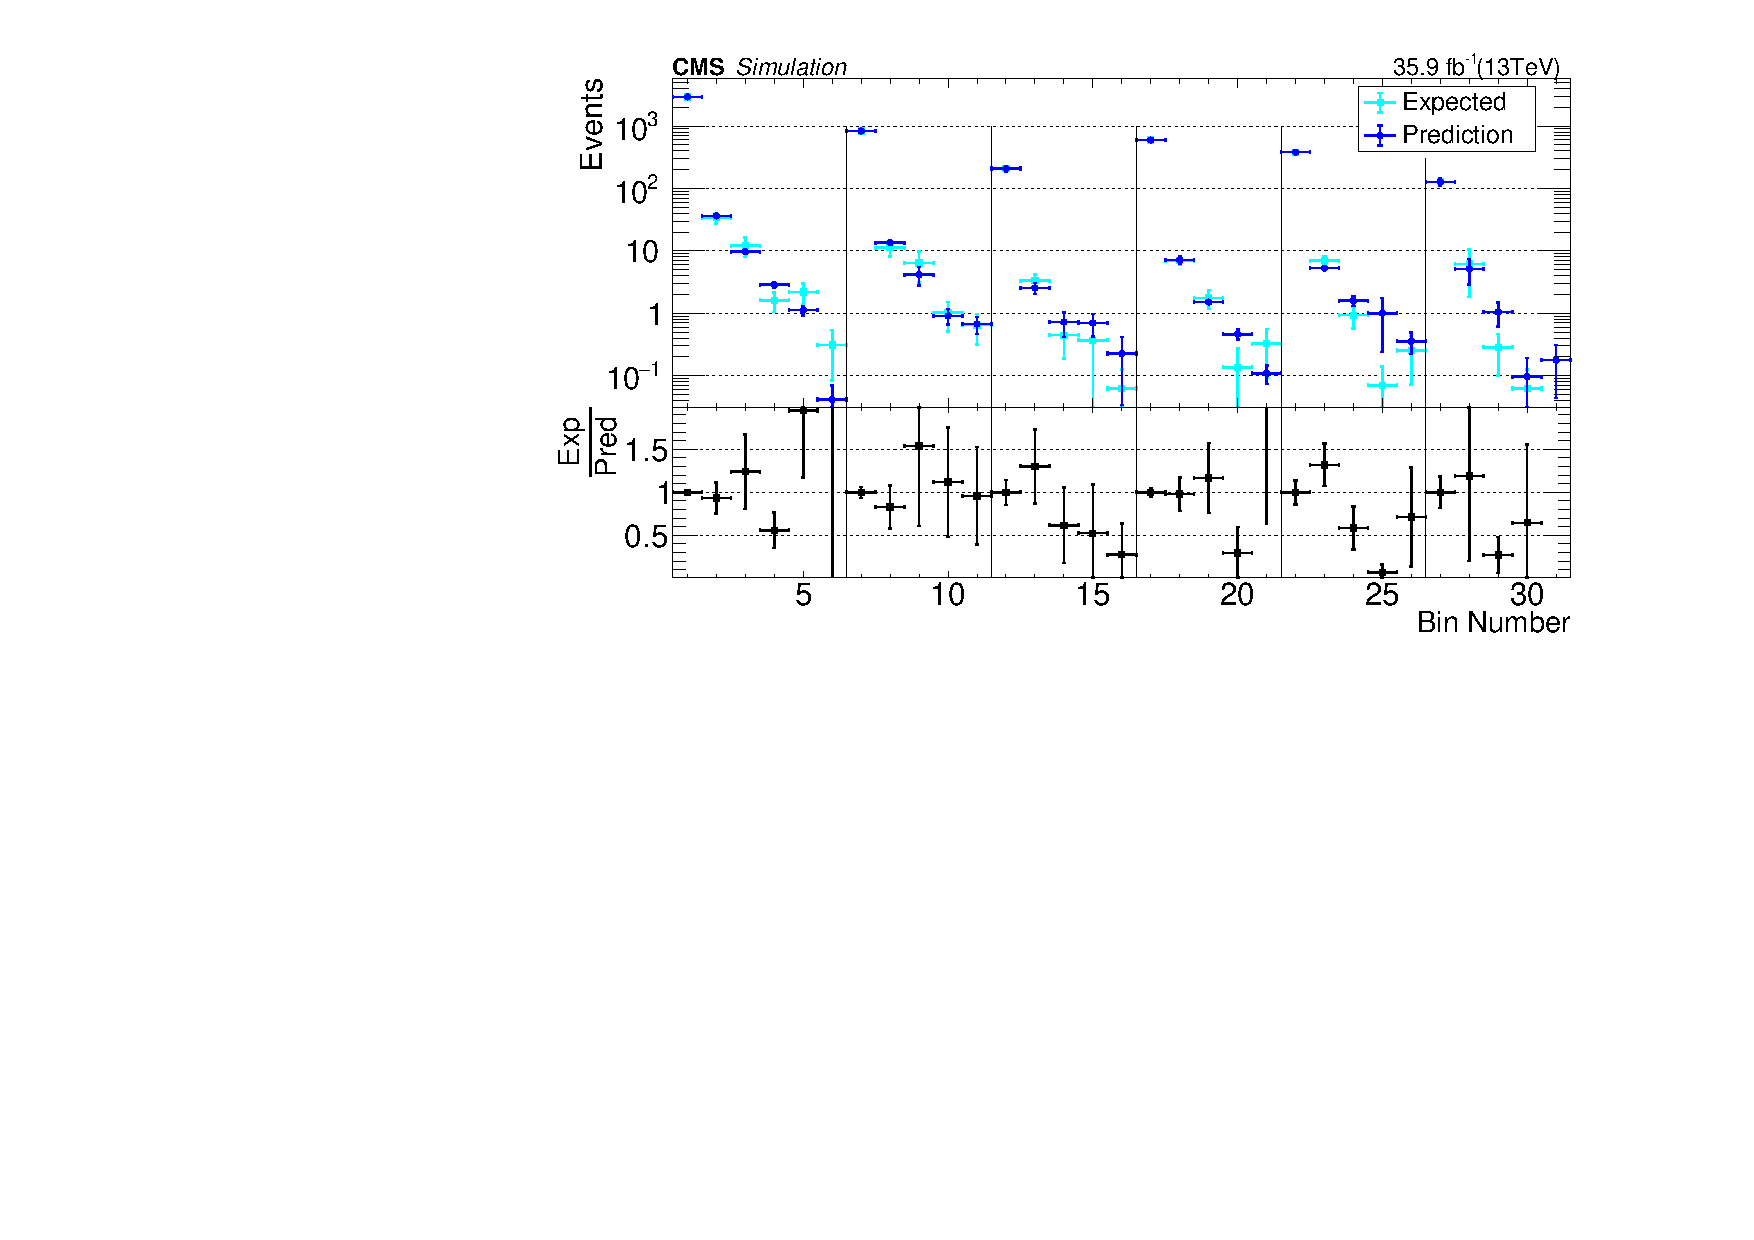
\includegraphics[width=0.85\linewidth]{../Figures/Chap3/SUSY_Photon_MET_JbJ_18Aug17/FakeMET/SBins_v4_prompt_doubleR_SRselection.pdf}
\caption[Closure for \gjets and QCD multijet]{Comparison of \gjets and QCD multijet background estimated using low-\dphi control regions taken from MC (blue) to that expected in search regions (cyan).}
\label{fig:qcdclosure}
\end{figure}

\begin{table}[h!]
\centering
\caption[Double ratio in data and MC for validation region]{Double ratio($\kappa^{\text{MC}}$) computed in the one $\gamma$ regions and ratio of high-$\dphi$ to low-$\dphi$ ($R^{data}$) obtained from data using 100 $<$ \ptmiss $<$ 200~\gev region with electroweak contribution subtracted.}
\label{tab:qcdDoubleRatioPhoton}
\begin{tabular}{c|c|c|c}
\nb & \nj  & $K^{\text{MC}}$ & $R^{data}$\\\hline\hline
\multirow{3}{*}{0} & 2 - 4   &  0.29  $\pm$  0.04   &   0.80 $\pm$  0.02 \\
   & 5 - 6   &  0.47  $\pm$  0.11   &   0.94 $\pm$  0.05 \\
   &$\geq 7$ &  0.40  $\pm$  0.11   &   1.04 $\pm$  0.17 \\ \hline
\multirow{3}{*}{$\geq 1$} & 2 - 4   &  0.24  $\pm$  0.05   &   0.65 $\pm$  0.03 \\
   & 5 - 6   &  0.34  $\pm$  0.07   &   0.91 $\pm$  0.09 \\
   &$\geq 7$ &  0.47  $\pm$  0.34   &   1.29 $\pm$  0.26 \\ \hline
\end{tabular}
\end{table}

Since the double ratio $\kappa$(\nj,\nb) used for correcting R in low and high \ptmiss regions is obtained from MC, and makes an important component of this method, it is validated using data. To define the data control sample, photon selection is inverted and events with a well identified photon are vetoed. In these zero photon events, the jet with the highest electromagnetic fraction is used as a proxy to the photon, and all baseline selection criteria are applied to the event. The jet used as proxy-photon is removed from the list of jets to avoid any double counting of the objects. With this zero photon event sample, double ratio, $\kappa$(\nj,\nb), is calculated exactly as in MC events. 

The zero photon control sample is obtained from the data collected using a combination of inclusive \HT and single jet triggers as explained in~\ref{sec:triggers}. The electroweak contribution to this sample is subtracted using event yields from the MC simulation samples. The MC event yields are corrected for the trigger efficiencies. Since these triggers achieve efficiency plateau only for \HT$>$1 TeV, the \HT$>$1 TeV region is used for validating the double ratio. The closure of this validation method in MC is shown in Figure \ref{fig:no_photon_closure}. 
\begin{figure}[h!]
\centering
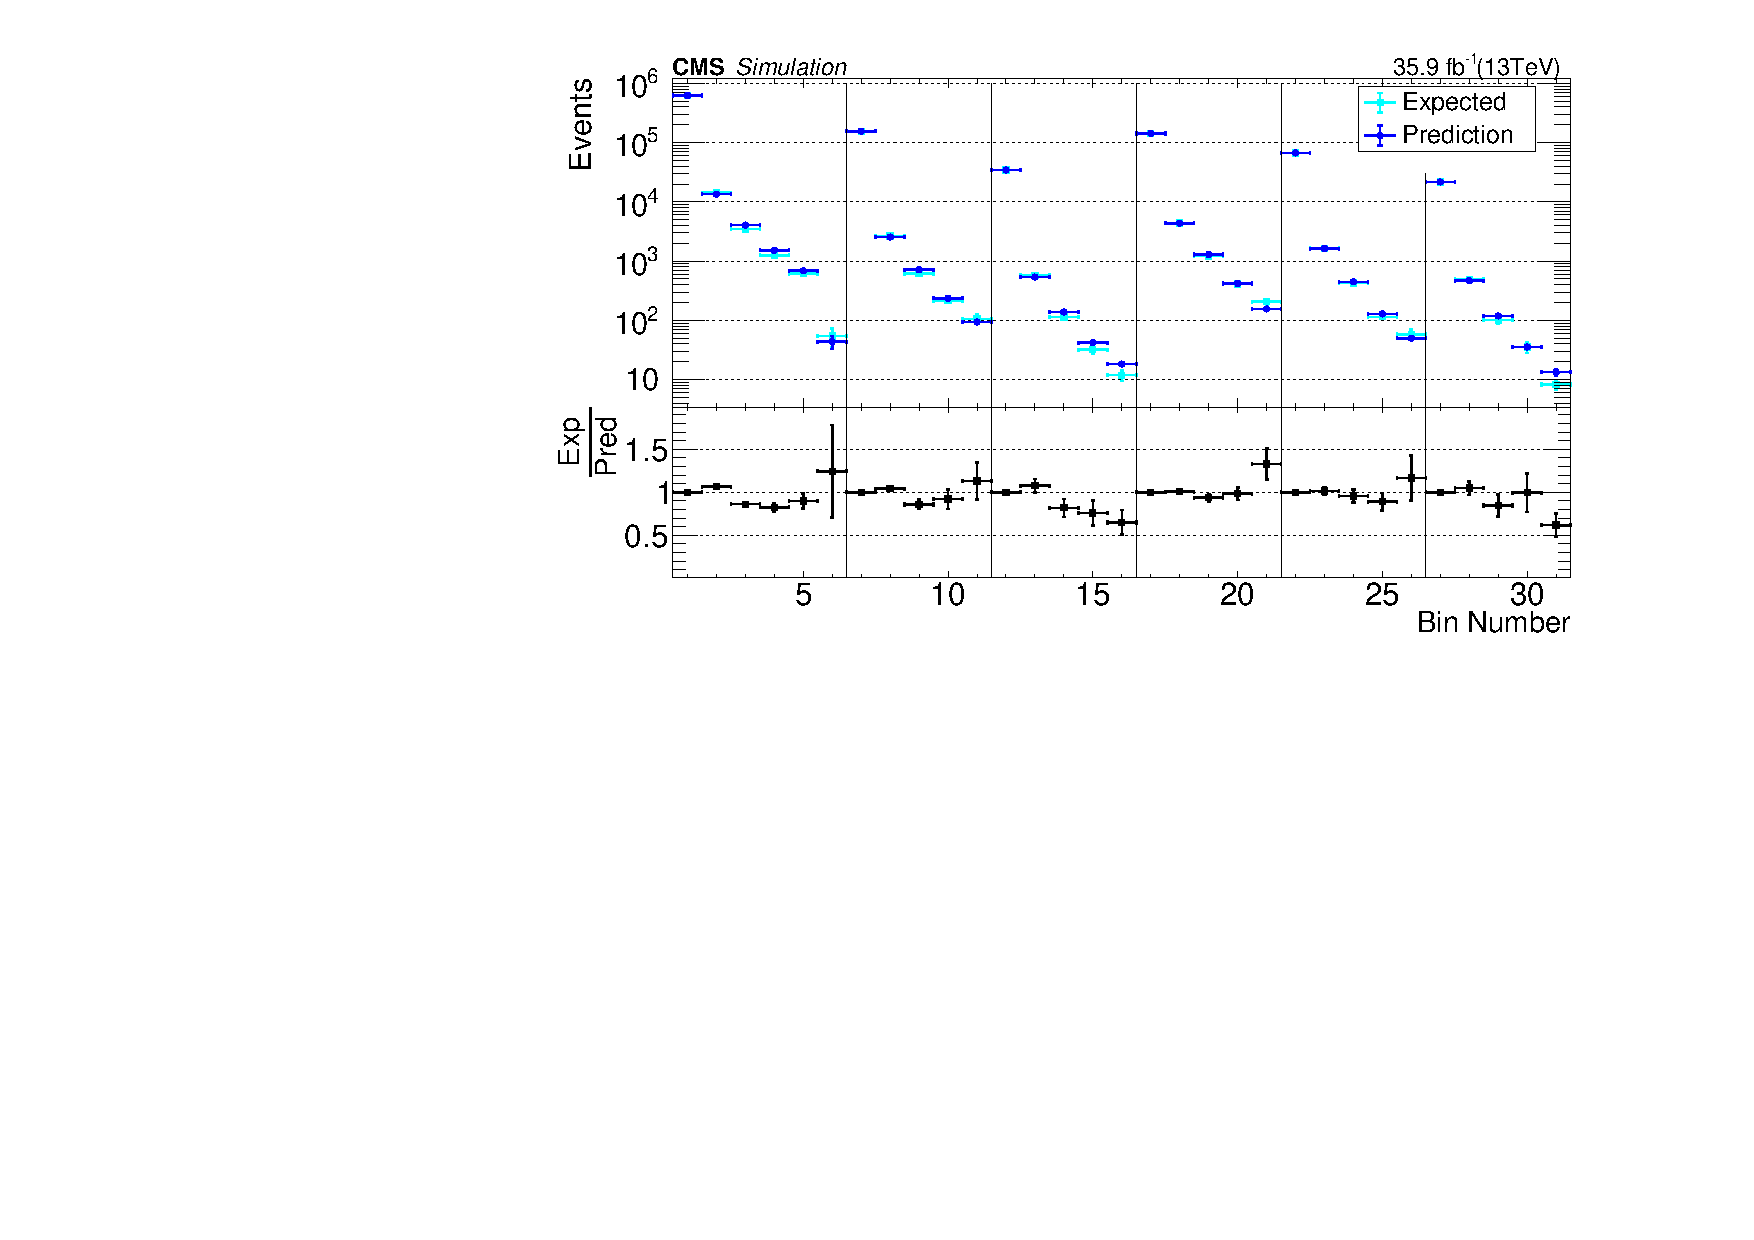
\includegraphics[width=0.85\linewidth]{../Figures/Chap3/SUSY_Photon_MET_JbJ_18Aug17/FakeMET/doubleR_ST1000.pdf}
\caption[Closure for VR]{In zero photon validation region in MC, comparison of \gjets and QCD multijet background estimated using low-\dphi control regions taken from MC (blue) to that expected in search regions (cyan).}
\label{fig:no_photon_closure}
\end{figure}

The values of double ratio, $\kappa$(\nj,\nb) obtained from zero photon validation region in data and MC are compared in Figure \ref{fig:Figure_003}.
\begin{figure}[h!]
\centering
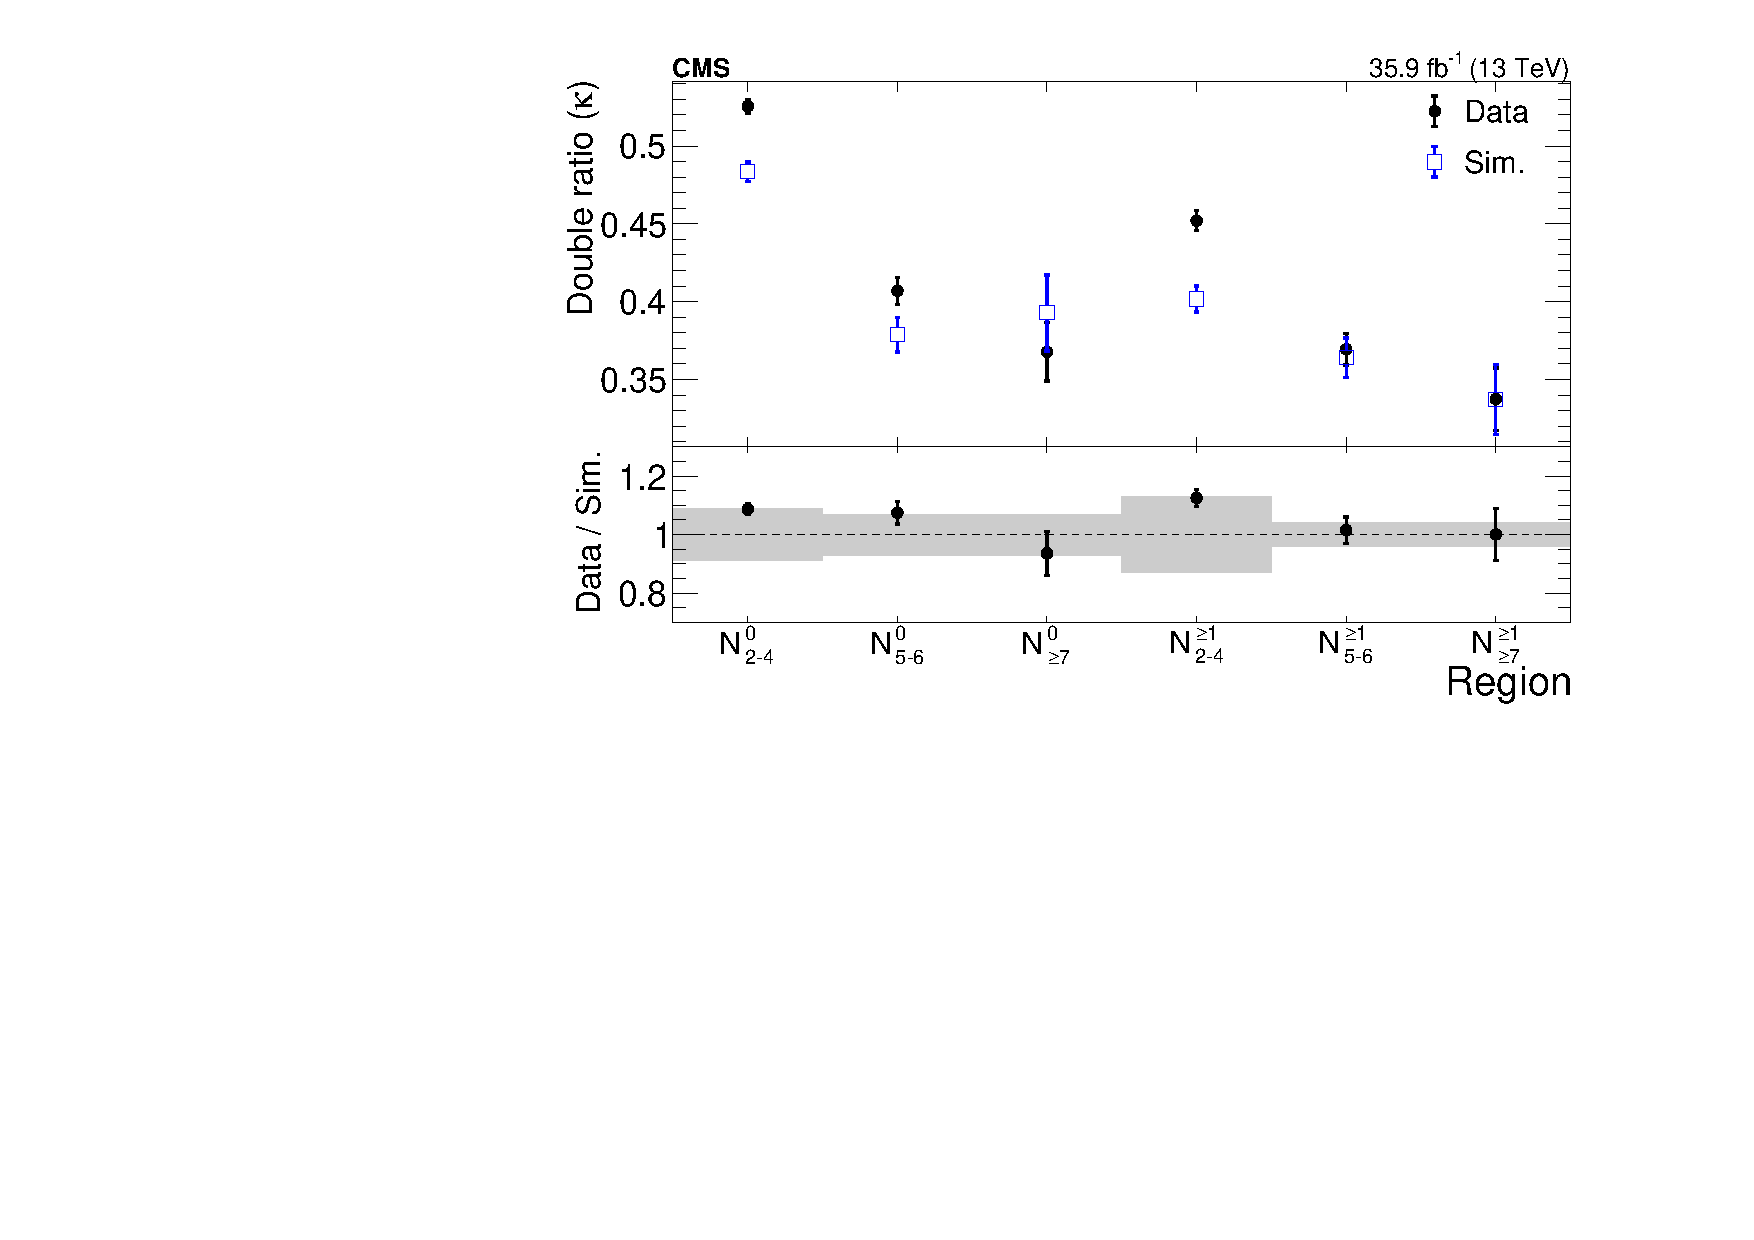
\includegraphics[width=0.8\linewidth]{../Figures/Chap3/anaPublic/Figure_003}
\caption[Double ratio validation]{The double ratio $\kappa$ in each \nj-\nb region for
zero-photon events. The filled black circles are the observed $\kappa$ values after subtracting
the electroweak contamination based on simulation. The open blue squares are the
$\kappa$ values computed directly from simulation.  The ratio is shown in the bottom
panel, where the shaded region corresponds to the systematic uncertainty in the \gjets prediction.
In the label \njb, j refers to the number of jets and b refers to the number of b-tagged jets.}
\label{fig:Figure_003}
\end{figure}

The uncertainties on predicted \gjets and QCD multijet background is dominated by statistical size of event sample in low-\dphi control region with \ptmiss $>$ 200~\gev i.e. the region B, and ranges from 6-100\%. These components of systematic uncertainties are taken uncorrelated across all bins. An additional contribution to this control region is due to uncertainties on predicted electroweak backgrounds which is subtracted from region B. This can range between 10-100\%.  Since R(\nj, \nb) = high-\dphi/low-\dphi is defined in the bins of \nj and \nb from low \ptmiss sideband in single photon side band, statistical uncertainties on R are taken to be correlated for all bins with same \nj and \nb. The uncertainties on double ratio have two components: (a) difference between $K_{0\gamma}$ in data and MC, and (b) statistical uncertainty on $K_{0\gamma}^{\text{MC}}$. These two contributions are added in quadrature to assign the systematic uncertainties which are also taken fully correlated for all bins with same \nj and \nb.
The final predictions of \gjets and QCD multijet processes is shown in \ref{tab:qcdPrediction}.

